\documentclass[uplatex, a4paper, 12pt, openany, oneside]{jsbook}

\usepackage[dvipdfmx]{graphicx}
\usepackage[dvipdfmx]{color}
\usepackage[dvipdfmx, bookmarks=true, setpagesize=false, hidelinks]{hyperref}
\usepackage{pxjahyper}

\usepackage{thesis}
\usepackage{here}
\usepackage{url}

\usepackage[hang,small,bf]{caption}
\usepackage[subrefformat=parens]{subcaption}
\captionsetup{compatibility=false}

\thesis{卒 業 論 文}
\title{
  \centering
    \scalebox{1.0}{測域センサの反射強度を利用した視覚と行動の}\\
    \vspace{-0.3zh}
    \scalebox{1.0}{end-to-end学習による人追従行動の模倣}\\
    \vspace{-0.3zh}

    \scalebox{0.7}{Imitation-based end-to-end learning for human tracking behavior}\\
    \vspace{-0.6zh}
    \scalebox{0.7}{using reflected intensity from range sensors}\\
    \vspace{-0.6zh}
}
\setlength{\textwidth}{\fullwidth}
\setlength{\evensidemargin}{\oddsidemargin}

\date{\today}
\vspace{-15.0zh}
\teacher{林原 靖男 教授}
\vspace{-15.0zh}
\organization{千葉工業大学 先進工学部 未来ロボティクス学科}
\author{20C1102 馬場 琉生}
% \vspace{-15zh}

\renewcommand{\baselinestretch}{1.2}
\begin{document}

%% Front Matter
\frontmatter{}
%
\maketitle
%
%!TEX root = ../thesis.tex
\chapter*{概要}
\thispagestyle{empty}
%
\begin{center}
  \scalebox{1.5}{ラグランジュ法}\\
\end{center}
\vspace{1.0zh}
%
 三次元空間で運動する場合,並進運動と回転運動の 2 つの成分に分けられる.並進運動
はニュートンの運動方程式,回転運動はオイラーの運動方程式で記述することができ,こ
れらを合わせてニュートン・オイラー法と呼ぶ.ニュートン・オイラー法を利用すること
で,各リンクの重心に作用する力とトルクを計算することができる.この代替手法とし
て,ラグランジュ法が挙げられる.ラグランジュ法は,エネルギベースのアプローチで,
剛体リンクを備えた直動マニピュレータにある程度特化している.
\vspace{1.0zh}

キーワード: ラグランジュ,運動エネルギ,位置エネルギ

%
\tableofcontents
%
\listoffigures
%
% \listoftables
%

%
%% Main Matter
\mainmatter{}
%
\chapter{序論}
\label{chap:introduction}
%
%\input{introduction/preface}
%
%!TEX root = ../thesis.tex

\section{背景}
近年,機械学習を用いた自律移動に関しての研究が盛んに行われている.本研究室でも,機械学習を用いた画像に基づく人追従行動の生成に関する研究を行ってきた.

パシンら\cite{pasin1}\cite{pasin2}\cite{pasin3}は,引き紐を利用して画像に基づく人追従行動を生成する手法を提案している.これは,深層強化学習\cite{hado}を用いており,引き紐に取り付けられたポテンショメータでリンクの角度を取得し,それに応じた報酬をエージェント(ロボット)に与えて強化学習\cite{leslie}することで,画像に基づいて人追従する行動を生成できることを示した.
\figref{Fig:pasin_system}にシステムの概要を示す.入力は画像で,出力は直進,左旋回,右旋回のいずれかの行動である.報酬は,引き紐を取り付けたリンクの角度に基づいており,人がロボットの正面に立つと報酬が高くなるように設定されている.ロボットは報酬が高くなるように行動を選択するため,引き紐を持つ人がロボットの正面にいない場合は,引き紐を持つ人がロボットの正面になるように,左旋回や右旋回といった行動を選択する.引き紐を持つ人が正面にいる場合は,ロボットは直進を選択する.さまざまな行動と画像に対して,リンクの角度に応じた報酬を与えることで,徐々に人を追従する適切な行動を選択していった.
しかし,強化学習の特性により,行動の選択がランダムに探索される場合がある.その結果,報酬の低い行動が選択され,追従対象者が望まない行動が発生する可能性がある.また,カメラ画像に基づく人追従行動を獲得するまでに約20分かかり,その間にロボットは望まない行動を繰り返すため,追従対象者に比較的負担がかかるという問題があった.

  \begin{figure}[h]
    \centering
    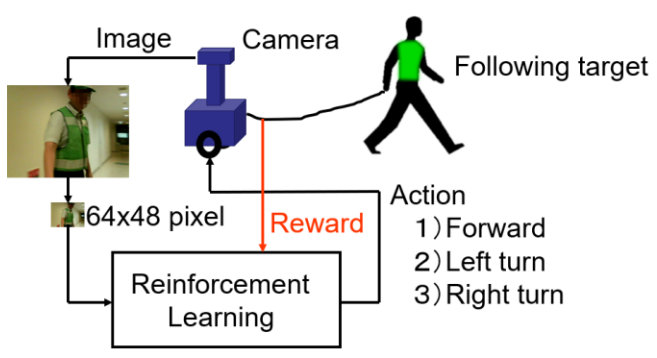
\includegraphics[keepaspectratio, scale=0.45] {images/pasin_system.png}
    \caption{Proposed method \cite{pasin1}}
    \label{Fig:pasin_system}
  \end{figure}

岡田ら\cite{okada}は,強化学習のような教師なし学習ではなく,深層学習\cite{yann2}という教師あり学習を用いて画像に基づく人追従行動を生成する手法を提案している.これは,後述するBojarskiら\cite{bojarski}の技術(end-to-end学習)を人追従問題に応用しており,強化学習を使用していないため,ロボットの行動がランダムに選択されることはない.また,学習時はルールベース制御器でロボットを制御しているので,常に人を追従する.つまり,学習時にも人追従行動を獲得することができ,強化学習を採用する手法と比べて追従対象者の負担が少ないというメリットがある.
\figref{Fig:okada_system}にシステムの概要を示す.まず,学習時は,追従対象者が引き紐を操作する.引き紐には同じくポテンショメータが取り付けられていて,ヨ―関節の変位角が0度となるようにロボットは直進や左旋回,右旋回のいずれかの行動で制御される.並行して,これらの行動とカメラ画像を深層学習器にオンラインでend-to-end学習する.学習後は,追従対象者が引き紐を操作しなくても,深層学習器によりカメラ画像を入力するだけで,出力は直進や左旋回,右旋回といった行動を選択する.つまり,学習時のルールベース制御器(引き紐による人追従行動)を模倣するように深層学習器(カメラ画像による人追従行動)は振る舞う.

  \begin{figure}[h]
    \centering
    \begin{minipage}[c]{100mm} 
        \centering
        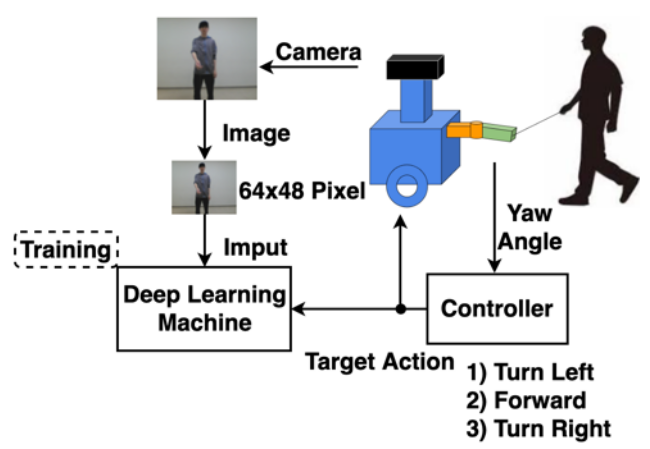
\includegraphics[width=100mm]{images/okada_learning_phase_system.png}
        \subcaption{Learning phase}
    \end{minipage} \\
    \vspace{1em} % 画像とキャプションの間にスペースを追加
    \begin{minipage}[c]{100mm} 
        \centering
        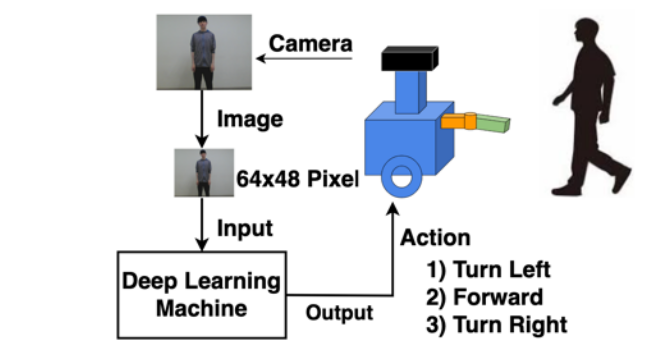
\includegraphics[width=100mm]{images/okada_following_phase_system.png}
        \subcaption{Following phase}
    \end{minipage}
    \caption{The proposed method for learning of the person-following behavior\cite{okada}}
    \label{Fig:okada_system}
  \end{figure}
% \subsection{etc...}
% \subsubsection{etc...}

\newpage

%!TEX root = ../thesis.tex

\section{関連研究}
     Bojarskiら\cite{bojarski}は,カメラ画像と人が操作するステアリングの角度を用いて模倣学習を行うことで,自動車の自動運転に成功している.学習時のシステムを\figref{Fig:bojarski_train}に示す.学習時には,ドライバーが車を運転し,その際に取得したステアリングの角度とカメラ画像を組み合わせてend-to-end学習が行われる.
     これにより,学習後は,\figref{Fig:bojarski_test}に示ようにカメラ画像から直接,ステアリングの角度を出力するシステムになっている.すなわち,カメラ画像のみで自動運転を可能にしている.
     
     \begin{figure}[h]
          \centering
          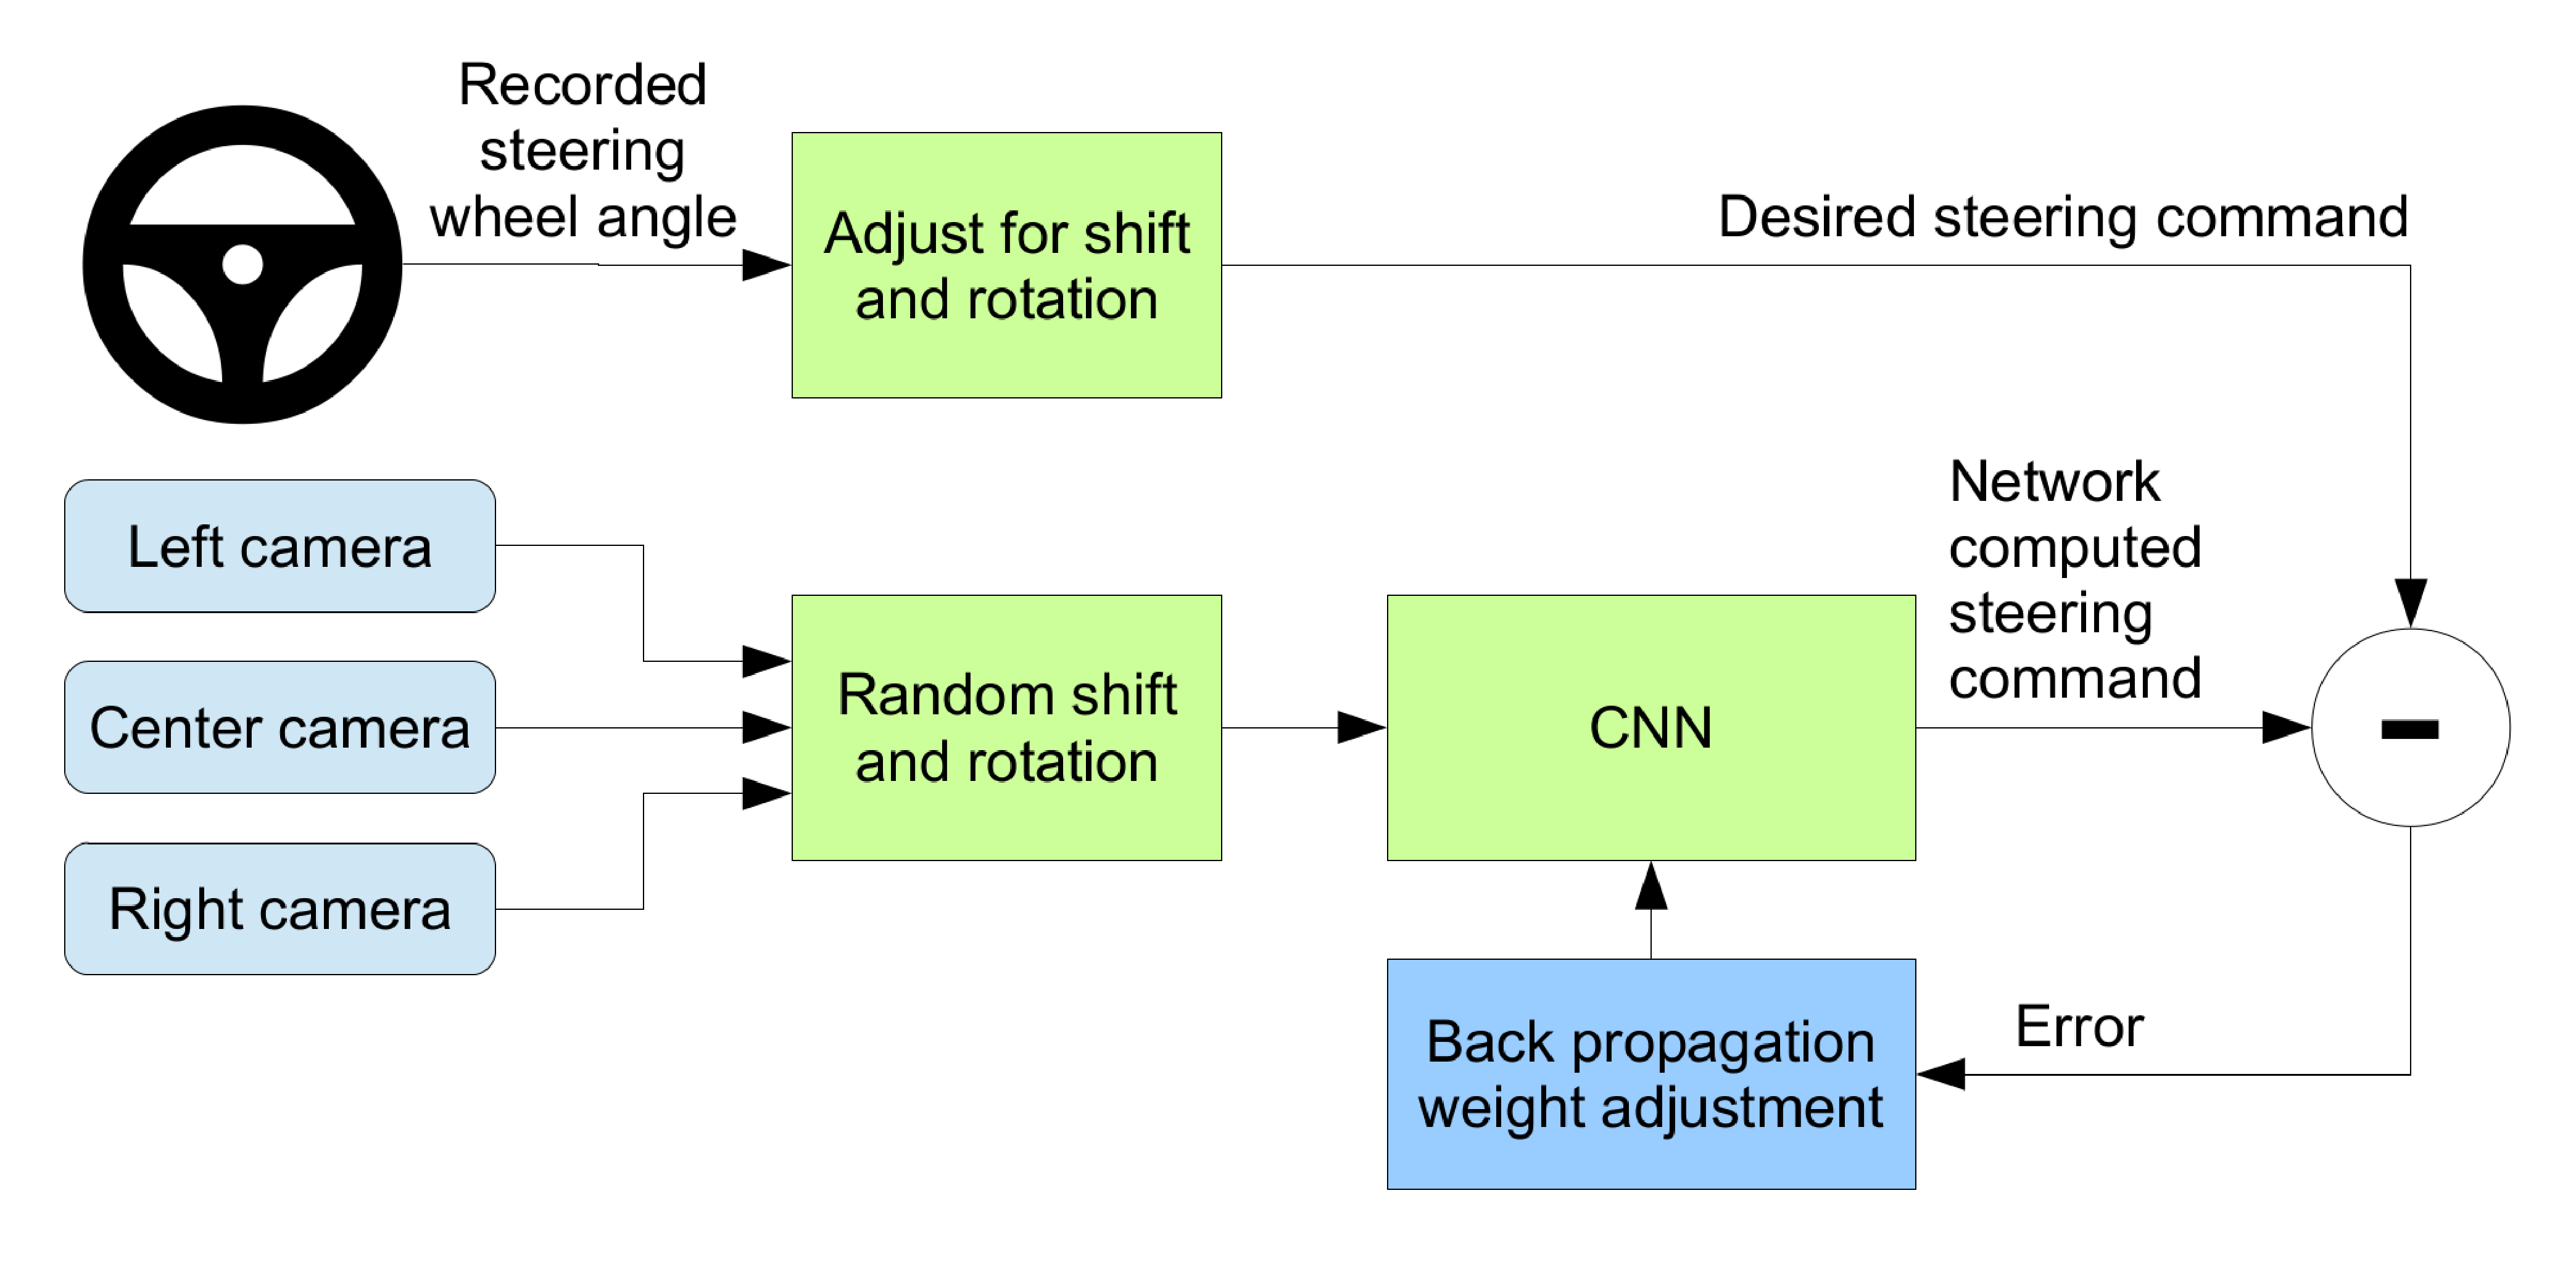
\includegraphics[keepaspectratio, scale=0.16] {images/eps/bojarski_train}
          \caption[Training the neural network]{Training the neural network (source: \cite{bojarski})}
          \label{Fig:bojarski_train}
     \end{figure}



     \begin{figure}[h]
          \centering
          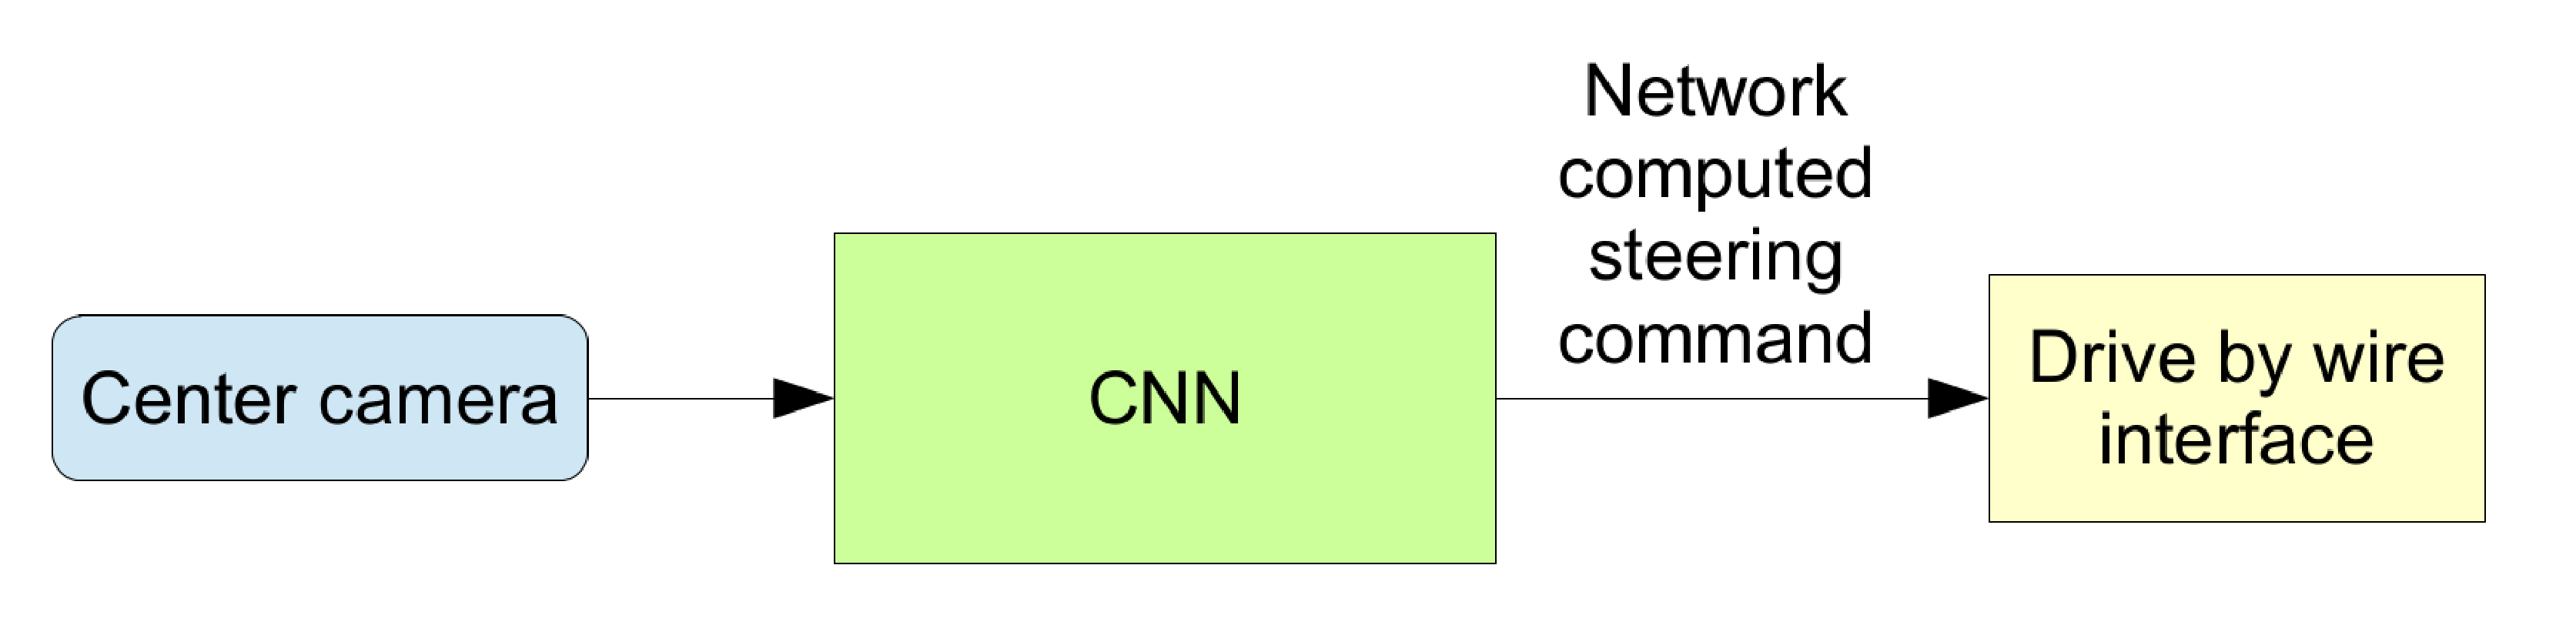
\includegraphics[keepaspectratio, scale=0.20] {images/eps/bojarski_test.eps}
          \captionsetup{justification=raggedright} % キャプションを左寄せに
          \caption[The trained network is used to generate steering commands from a single front-facing center camera.]{The trained network is used to generate steering commands from a single front-facing center camera. (source: \cite{bojarski})}
          \label{Fig:bojarski_test}
     \end{figure}

\newpage

     \figref{Fig:bojarski_CNN}は,CNNが白線等のない未塗装道路においても,人が操作するステアリングの角度だけを教師信号として用い,有用な道路の特徴を学習したことを示している.なお,道路の輪郭を検出するような学習は明示的に行っていないことが述べられている.

     \begin{figure}[h]
          \centering
          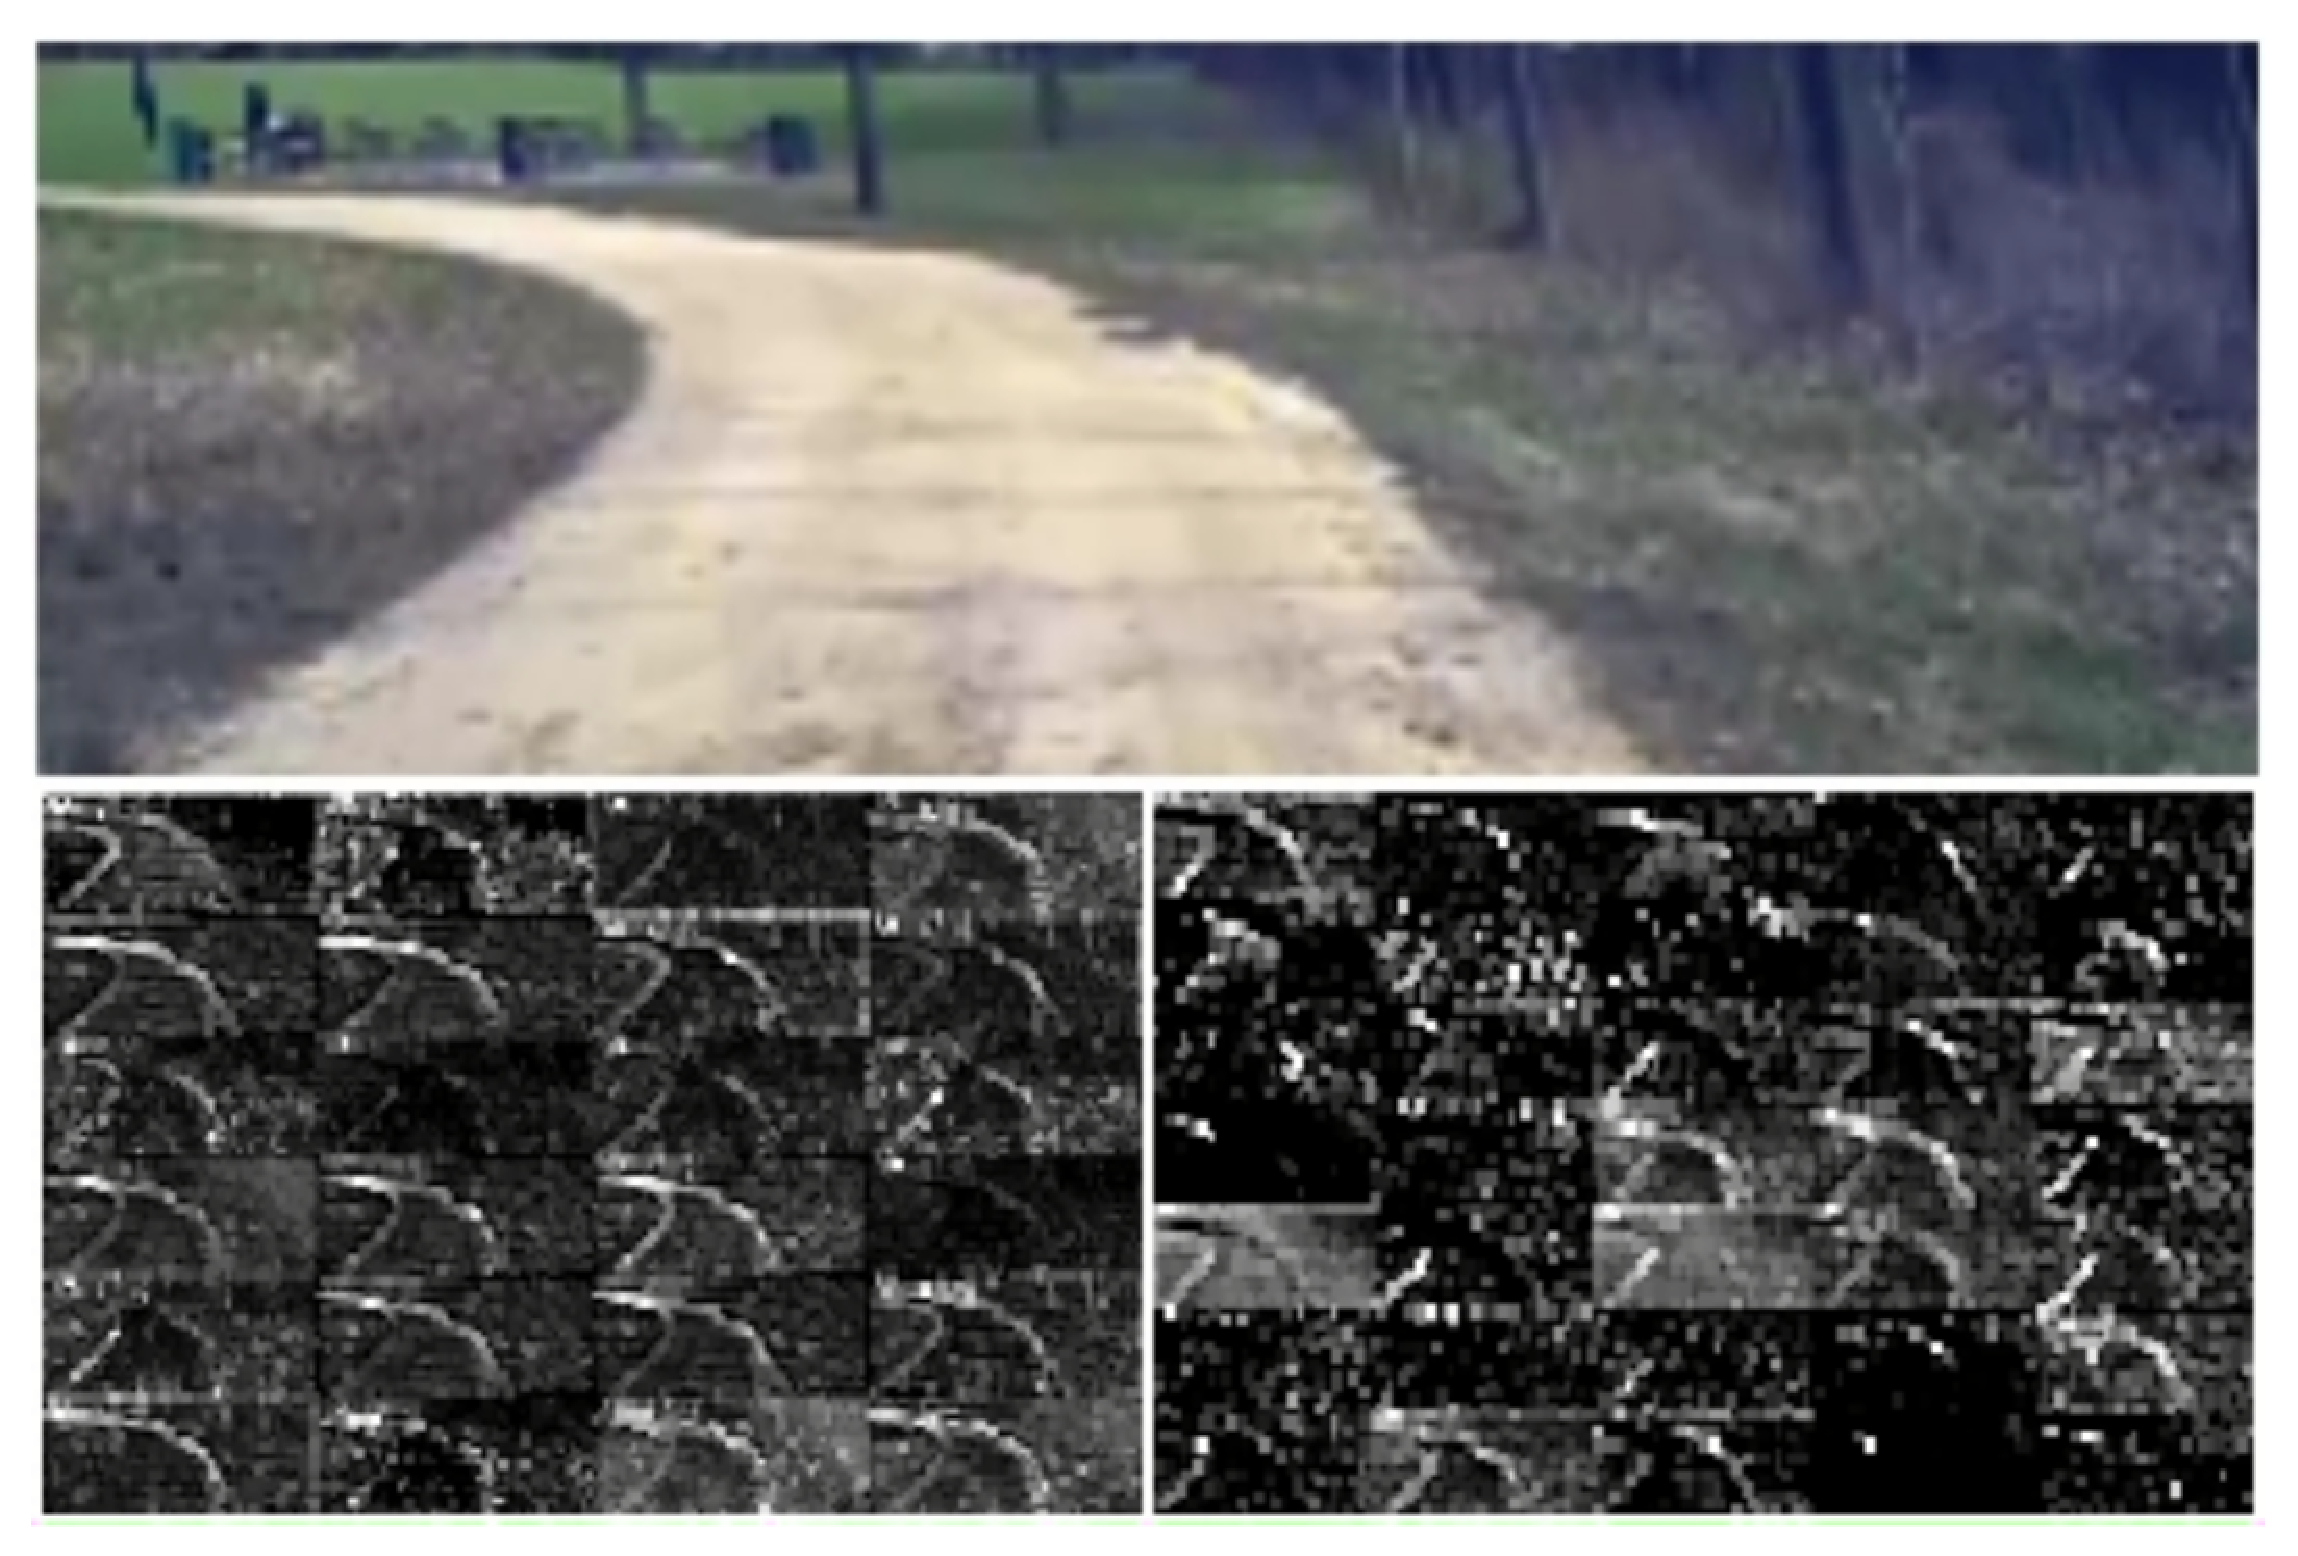
\includegraphics[keepaspectratio, scale=0.35] {images/eps/bojarski_CNN.eps}
          \captionsetup{justification=raggedright} % キャプションを左寄せに
          \caption[How the CNN ``sees'' an unpaved road. Top: subset of the camera image sent to the CNN. Bottom left: Activation of the first layer feature maps. Bottom right: Activation of the second layer feature maps. This demonstrates that the CNN learned to detect useful road features on its own, i.e., with only the human steering angle as training signal. We never explicitly trained it to detect the outlines of roads.]{How the CNN ``sees'' an unpaved road. Top: subset of the camera image sent to the CNN. Bottom left: Activation of the first layer feature maps. Bottom right: Activation of the second layer feature maps. This demonstrates that the CNN learned to detect useful road features on its own, i.e., with only the human steering angle as training signal. We never explicitly trained it to detect the outlines of roads. (source: \cite{bojarski})}
          \label{Fig:bojarski_CNN}
     \end{figure}

\newpage

%!TEX root = ../thesis.tex

\section{目的}

本研究では, 2DLiDARの反射強度を利用したルールベース制御器による人追従行動をカメラ画像を用いて end-to-end 学習して模倣する手法を提案し, カメラ画像に基づいた人追従行動が可能か, 実ロボットを用いた実験によりその有効性を検証する.

\newpage

%!TEX root = ../thesis.tex

\section{論文の構成}

  第1章では,本研究の背景,目的,関連研究について述べた.第2章では,本研究で用いる要素技術について述べる.第3章では,本研究の提案手法を述べる.第4章では,提案手法を用いた実験を行う.第5章では,本研究の結論を述べる.

\newpage

%

%ここにディレクトリのパスを追加していく
\chapter{要素技術}

  本章では,本研究で用いた深層学習に関連した要素技術と,引き紐を用いたルールベース制御器,ベースとなる従来手法について述べる.

\label{chap:technology}
%
%!TEX root = ../thesis.tex

\section{深層学習}

  深層学習(Deep learning)は,画像や音声などの複雑なデータを処理するための機械学習手法であり,人工ニューラルネットワークを基盤としている.\figref{Fig:deep_neural_network}に示すように,多層のニューロンが組み合わさり,人間の脳のような階層的な構造をしている.これにより,例えば画像や音声の特徴を学習し,自動的に認識や分類を行うことが可能になる.

  \begin{figure}[h]
    \centering
    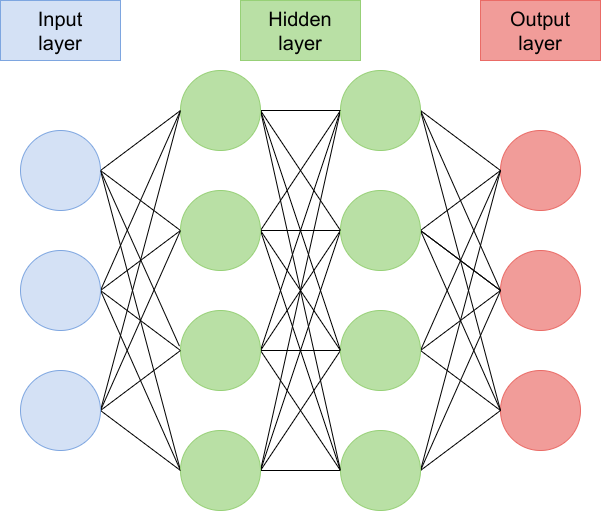
\includegraphics[keepaspectratio, scale=0.30] {images/deep_neural_network.png}
    \caption{Neural network}
    \label{Fig:deep_neural_network}
  \end{figure}

\newpage

\subsection{end-to-end学習}

  end-to-end学習は,\figref{Fig:about_end-to-end}に示すように,システムの入力から出力までの全体の処理を一つのニューラルネットワークで直接学習する機械学習手法である.この手法では,画像や音声などの特徴抽出や前処理の段階を人手で設計する必要がなく,データから直接目標のタスクを学習することができる.

  \vspace{2cm}

  \begin{figure}[h]
    \centering
    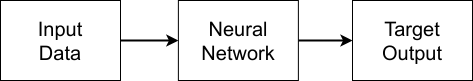
\includegraphics[keepaspectratio, scale=0.70] {images/RobotGuidance_about_end-to-end.png}
    \caption{Structure of end-to-end learning}
    \label{Fig:about_end-to-end}
  \end{figure}

  \vspace{1cm}

\subsection{ミニバッチ学習}

  本研究は,オンライン(データを収集しながら)でミニバッチ学習を行う.利点として,リアルタイムでのデータへの迅速な適応性が挙げられる.新しいデータが入手されるたびに,小さなバッチごとにモデルを即座に更新することで,変動する状況にリアルタイムで対応し,モデルの性能を最新かつ効果的に維持することが可能である.通常,データセット全体を一度に処理するバッチ学習と,一つずつのデータを処理するオンライン学習の中間に位置するアプローチである.本論文では,「オンラインで学習」と「オンライン学習」の使い分けに注意する.

\newpage

\subsection{Convolutional Neural Network (CNN)}

  本研究の学習器は畳み込みニューラルネットワーク(Convolutional Neural Network:CNN)で,これは画像認識などで用いられている\cite{yann1}\cite{alex}.畳み込み層とプーリング層を含む構造で,多次元配列の形式データを効率的に処理するように設計されている.例として,LeCunら\cite{yann1}は,畳み込み層とプーリング層を連続して接続するネットワークを用いることで,手書き文字を識別できることを示した(\figref{Fig:yann_CNN}).また,Krizhevskyら\cite{alex}は,深い畳み込みニューラルネットワークを用いることで,1000種類のクラスに分類できることを示し(\figref{Fig:deep_convolutional_neural_networks}),ILSVRC(ImageNet Large Scale Visual Recognition Challenge)2012で優勝した.

  CNNは,主に畳み込み層,プーリング層,および全結合層から構成される.以下に,それぞれの特徴を記す.

  \begin{enumerate}
    \item 畳み込み層\\
    入力データに対してフィルターを適用し,特徴を抽出した特徴マップを出力する層
    \item プーリング層\\
    特徴マップのサイズを削減し,特徴の位置に対する頑健性を向上させるために,領域内の最大値や平均値を取る操作を行う層
    \item 全結合層\\
    畳み込み層とプーリング層で抽出された特徴を組み合わせて,最終的な出力を生成する層
  \end{enumerate}

  \begin{figure}[h]
    \centering
    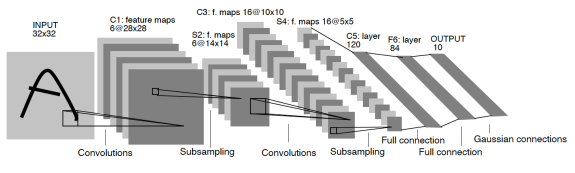
\includegraphics[keepaspectratio, scale=0.50] {images/yann_CNN.png}
    \caption[Training the neural network]{Training the neural network (source: \cite{yann1})}
    \label{Fig:yann_CNN}
  \end{figure}

\newpage

  \begin{figure}[h]
    \centering
    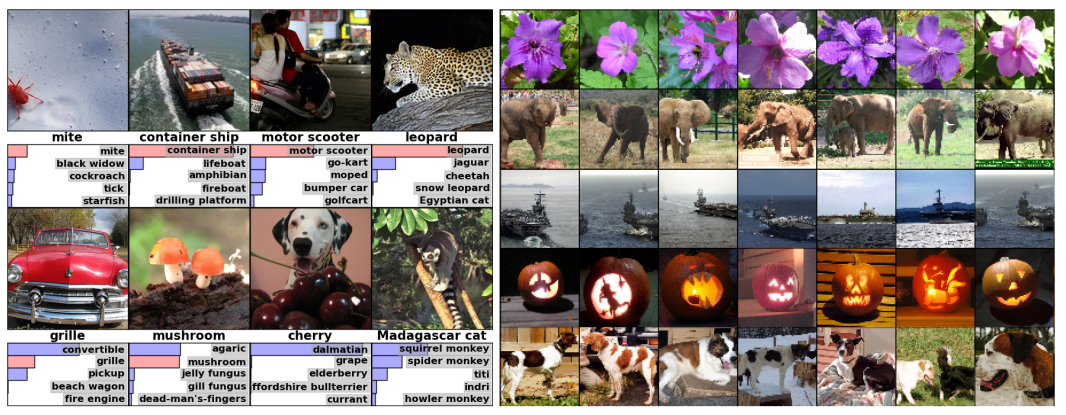
\includegraphics[keepaspectratio, scale=0.30] {images/deep_convolutional_neural_networks.png}
    \caption[ImageNet classification with deep convolutional neural network]{ImageNet classification with deep convolutional neural network (source: \cite{alex})}
    \label{Fig:deep_convolutional_neural_networks}
  \end{figure}


\newpage


%!TEX root = ../thesis.tex

\section{end-to-end学習}

\newpage

%!TEX root = ../thesis.tex

\section{Convolutional Neural Network (CNN)}

  本研究の学習器は畳み込みニューラルネットワーク(Convolutional Neural Network:CNN)で,これは画像認識などで用いられている\cite{yann1}\cite{alex}.畳み込み層とプーリング層を含む構造で,多次元配列の形式データを効率的に処理するように設計されている.例として,LeCunら\cite{yann1}は,畳み込み層とプーリング層を連続して接続するネットワークを用いることで,手書き文字を識別できることを示した(\figref{Fig:yann_CNN}).また,Krizhevskyら\cite{alex}は,深い畳み込みニューラルネットワークを用いることで,1000種類のクラスに分類できることを示し(\figref{Fig:deep_convolutional_neural_networks}),ILSVRC(ImageNet Large Scale Visual Recognition Challenge)2012で優勝した.

  CNNは,主に畳み込み層,プーリング層,および全結合層から構成される.以下に,それぞれの特徴を記す.

  \begin{enumerate}
    \item 畳み込み層\\
    入力データに対してフィルターを適用し,特徴を抽出した特徴マップを出力する層
    \item プーリング層\\
    特徴マップのサイズを削減し,特徴の位置に対する頑健性を向上させるために,領域内の最大値や平均値を取る操作を行う層
    \item 全結合層\\
    畳み込み層とプーリング層で抽出された特徴を組み合わせて,最終的な出力を生成する層
  \end{enumerate}

  \begin{figure}[h]
    \centering
    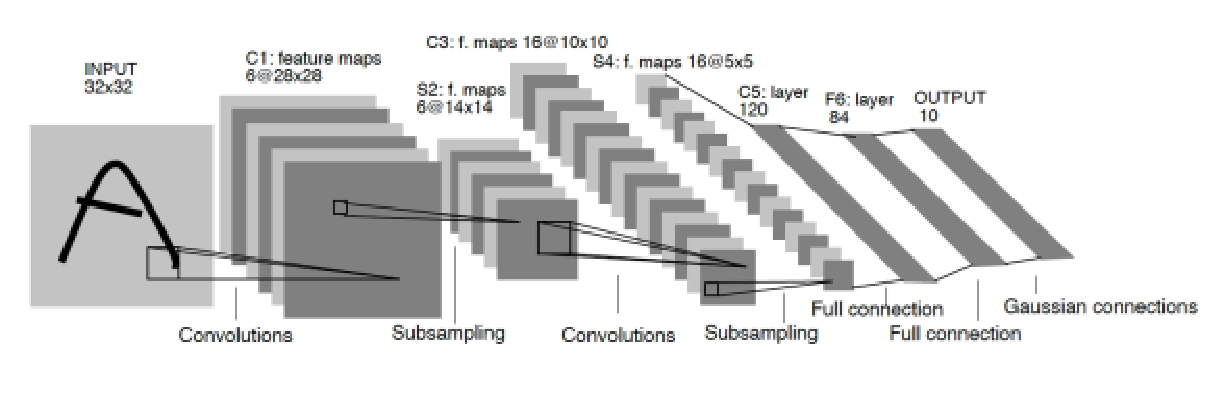
\includegraphics[keepaspectratio, scale=0.50] {images/eps/yann_CNN}
    \caption[Training the neural network]{Training the neural network (source: \cite{yann1})}
    \label{Fig:yann_CNN}
  \end{figure}

\newpage

  \begin{figure}[h]
    \centering
    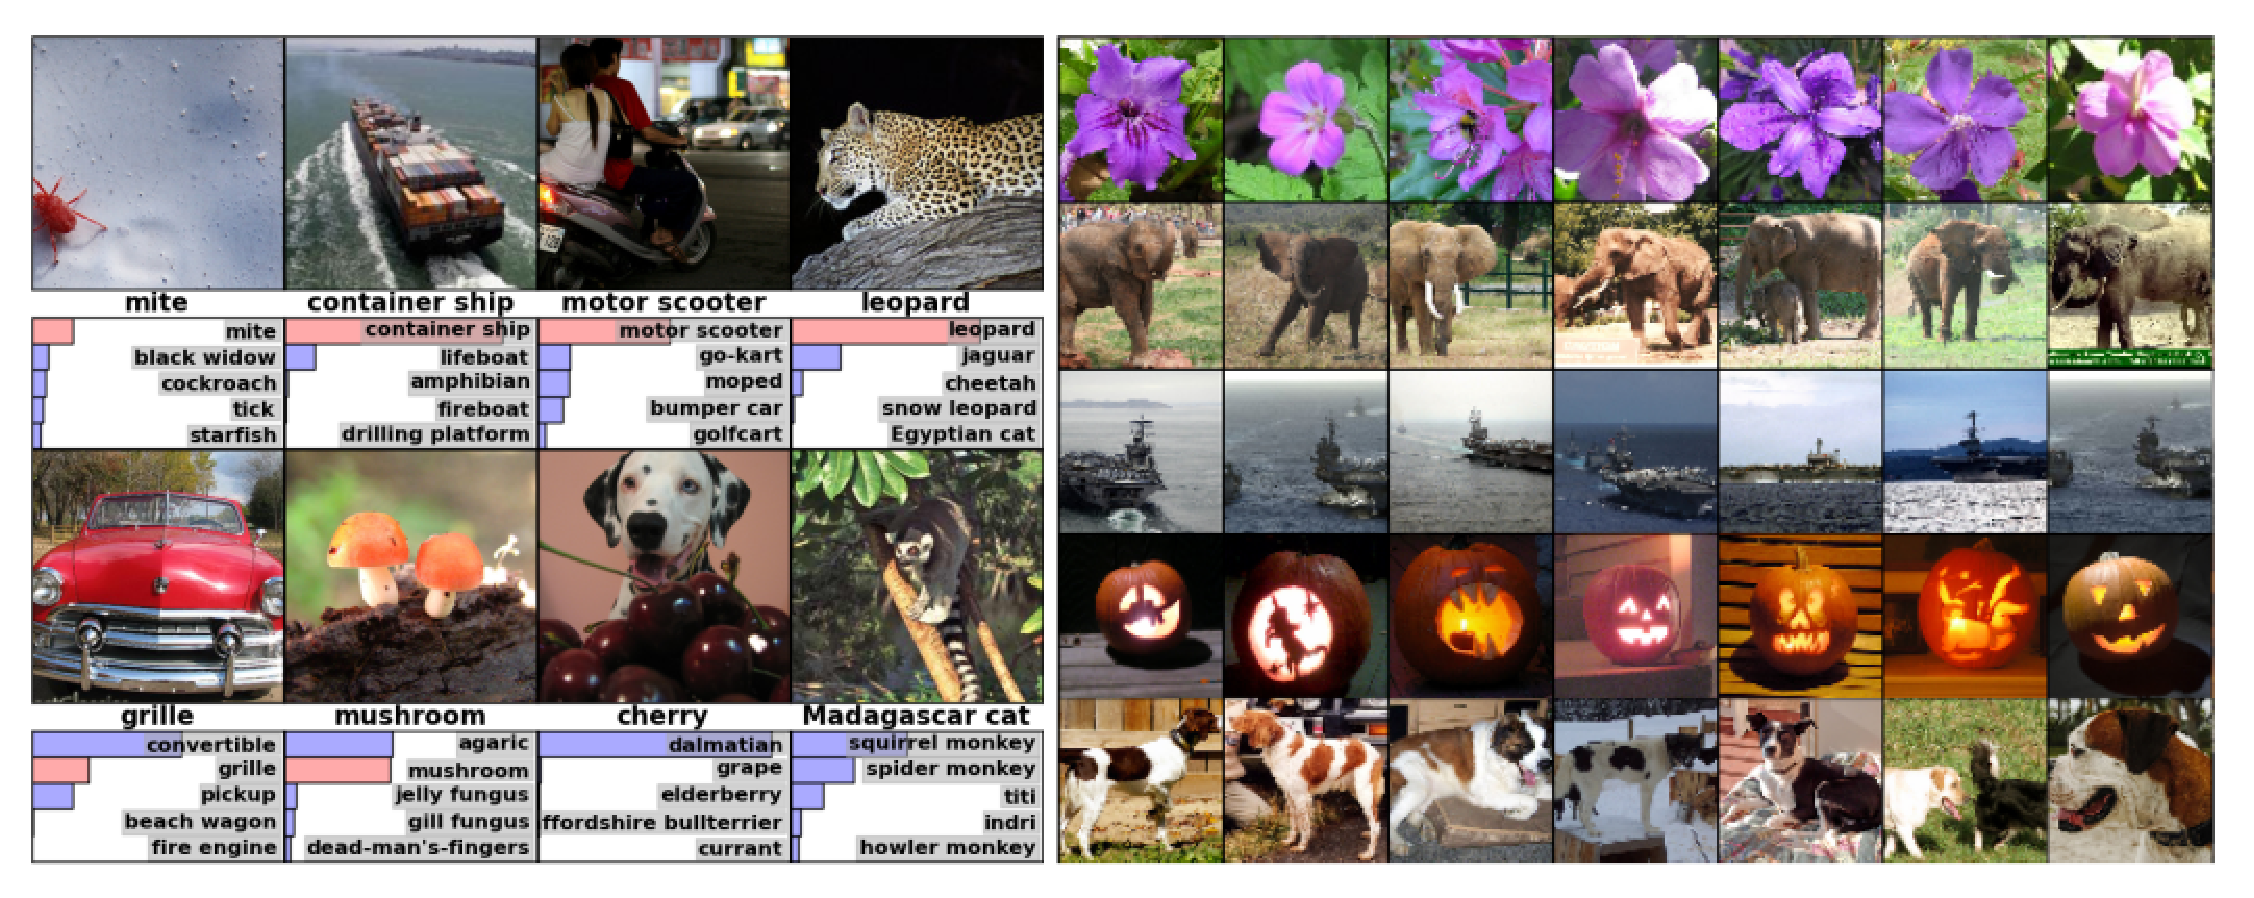
\includegraphics[keepaspectratio, scale=0.30] {images/eps/deep_convolutional_neural_networks}
    \caption[ImageNet classification with deep convolutional neural network]{ImageNet classification with deep convolutional neural network (source: \cite{alex})}
    \label{Fig:deep_convolutional_neural_networks}
  \end{figure}


\newpage

%!TEX root = ../thesis.tex

\section{ROS}

ROS(Robot Operating System)\cite{ros}は,オープンソースのロボットソフトウェアフレームワークであり,ロボットアプリケーションの開発や実行をサポートするミドルウェアである.異なるバージョンが存在しているが,本研究ではROS Noeticを使用している.

\subsection{LiDAR}

  LiDAR(Light Detection and Ranging)は,光を利用して距離を測定する技術であり,具体的には,レーザ光を発射し,対象物に当たって反射し戻ってくるまでの時間を計測することで距離を推定する.また,使用する装置によっては,物体によってどれだけの光が反射されたかを示す反射強度も測定することができる.したがって,LiDARは周囲の状況を把握し,環境認識や物体検知などに利用される.

  本研究で使用する2DLiDARを\figref{Fig:hokuyo_lidar}に示す.これは,北陽電機社製の2DLiDARであり,ROS上で\texttt{urg\_node}\cite{urg_node}というパッケージが提供されている.この\texttt{urg\_node}は,検出範囲(最大270 \,[deg])や反射強度の使用有無などのパラメータを変更するだけで簡単にデータのやり取りが可能である.

  \begin{figure}[h]
    \centering
    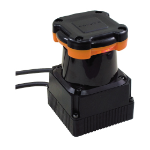
\includegraphics[keepaspectratio, scale=0.80] {images/RobotGuidance_hokuyo_lidar.png}
    \caption[Hokuyo 2DLiDAR (UTM-30LX)]{Hokuyo 2DLiDAR (UTM-30LX) (source: \cite{hokuyo})}
    \label{Fig:hokuyo_lidar}
  \end{figure}

\newpage

\subsection{RViz}

  RViz(ROS Visualization)\cite{rviz}は,ROSで提供される三次元ビジュアライゼーションツールであり,数値で表されるロボットの座標や各センサのデータ直感的に理解できる三次元空間上に表示することができる.\figref{Fig:RobotGuidance_rviz}にその様子を示す.ここでは,ロボットのモデルと2DLiDARからのセンサデータ,カメラ画像をリアルタイムに表示している.

  \begin{figure}[h]
    \centering
    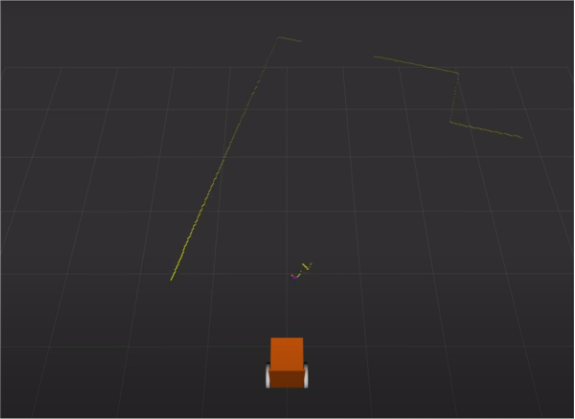
\includegraphics[keepaspectratio, scale=0.60] {images/RobotGuidance_rviz.png}
    \caption{RViz (Display robot model and scan data)}
    \label{Fig:RobotGuidance_rviz}
  \end{figure}

\newpage
%!TEX root = ../thesis.tex

\section{引き紐を用いたルールベース制御器}

\newpage


%

\chapter{提案手法}

  本章では,従来手法をベースとする提案手法の概要,提案手法における学習フェーズ,追従フェーズ,ルールベース制御器,ネットワーク構造についての5節に分けて述べる.

\label{chap:suggest}
%
%!TEX root = ../thesis.tex

\section{提案手法の概要}

  本研究は,ルールベース制御器の入力に引き紐ではなく,2DLiDARの反射強度を利用する.このときのロボットの行動を\figref{Fig:RobotGuidance_velocity}に示す.並進速度は,学習時と学習後で共に0.2 \,[m/s]で一定であり,ロボットのヨ―方向の角速度$\omega$のみが変化する.ルールベース制御器は,反射強度の高い方向にロボットを追従させる制御で,追従対象者に再帰反射テープを装着し,2DLiDARでそれを検出することで,人に追従する手法である.

  \begin{figure}[h]
    \centering
    \begin{minipage}[c]{65mm} 
        \centering
        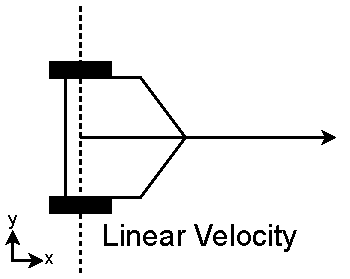
\includegraphics[height=40mm]{images/pdf/RobotGuidance_linear_velocity}
        \subcaption{Forward is fixed}
    \end{minipage}
    \begin{minipage}[c]{65mm} 
        \centering
        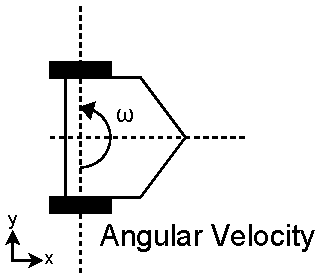
\includegraphics[height=40mm]{images/pdf/RobotGuidance_angular_velocity}
        \subcaption{Angular velocity changes depending on input}
    \end{minipage}
    \caption{Output robot actions}
    \label{Fig:RobotGuidance_velocity}
  \end{figure}

\newpage

  深層学習器は,ルールベース制御器の出力(ロボットのヨ―方向の角速度$\omega$)とRGB画像をend-to-end学習することで,\figref{Fig:RobotGuidance_simple_system}に示すように,入力をRGB画像,出力をロボットのヨ―方向の角速度$\omega$として人を追従する.

  \begin{figure}[h]
    \centering
    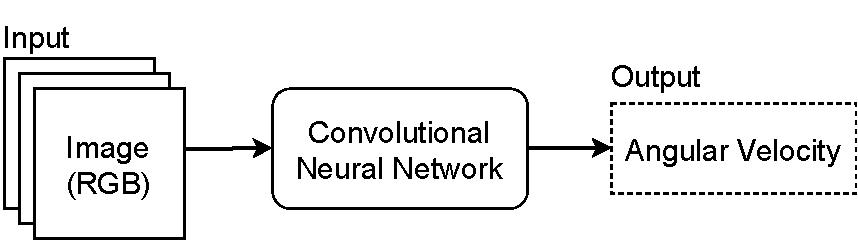
\includegraphics[height=3cm] {images/pdf/RobotGuidance_simple_system}
    \captionsetup{justification=raggedright} % キャプションを左寄せに
    \caption{The trained network is used to generate the robot's yaw angular velocity from the RGB images}
    \label{Fig:RobotGuidance_simple_system}
  \end{figure}

  \figref{Fig:RobotGuidance_all_system}に示すように,ルールベース制御器を用いてロボットを制御するフェーズを学習フェーズ,深層学習器の出力をロボットの行動にするフェーズをテストフェーズと呼ぶこととする.以下に,学習フェーズとテストフェーズの主な役割を示す.

  \subsubsection*{<学習フェーズ>}
  2DLiDARの反射強度を利用したルールベース制御器に従い,ロボットを制御する.制御器の出力と画像を教師信号として深層学習器に与え,オンラインでend-to-end学習する.
  
  \subsubsection*{<テストフェーズ>}
  2DLiDARは使用せず,画像を入力とした深層学習器の出力をロボットの行動にする.画像に基づいた人追従ができるかを実験により確認する.

  \begin{figure}[h]
    \centering
    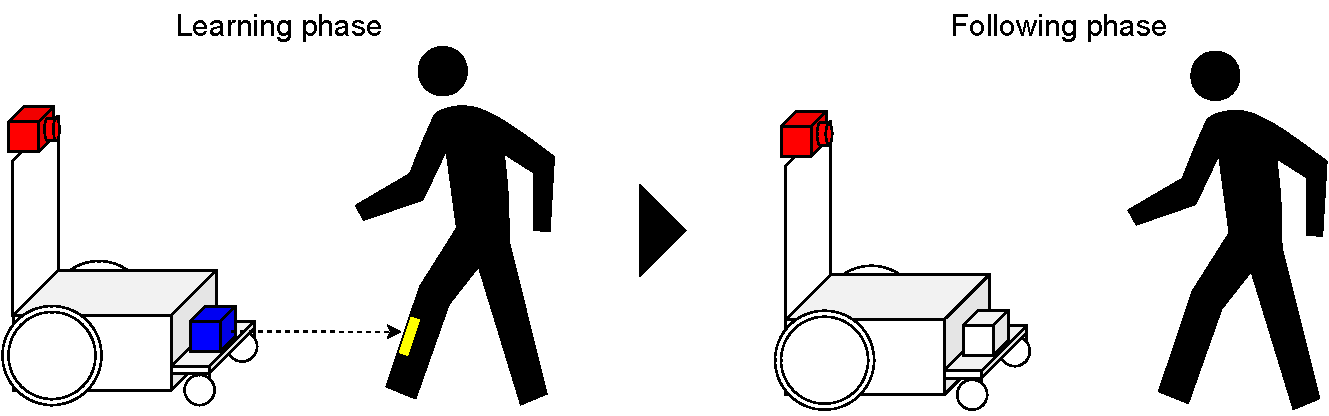
\includegraphics[height=3.5cm] {images/pdf/RobotGuidance_all_system}
    \captionsetup{justification=raggedright} % キャプションを左寄せに
    \caption{Sequence of proposed method}
    \label{Fig:RobotGuidance_all_system}
  \end{figure}

\newpage

%!TEX root = ../thesis.tex

\section{学習フェーズ}

  学習フェーズの概要を\figref{Fig:RobotGuidance_learning_system}に示す.学習フェーズでは,2DLiDARの反射強度を利用したルールベース制御器を用いて,\figref{Fig:RobotGuidance_learning_phase_leg}に示す追従対象者の足に装着した再帰反射テープに向かって,ロボットを制御する.ルールベース制御器の出力は,ロボットのヨ―方向の角速度$\omega$の1つとし,角速度$\omega$が0 \,[rad/s]となるようにロボットを制御することで人追従することが可能と考えられる.並行して,この行動とカメラの画像データを深層学習器に入力して,オンラインで学習させる.なお,並進速度は0.2 \,[m/s]で一定にしているため,深層学習器に入力しない.

  \begin{figure}[h]
    \centering
    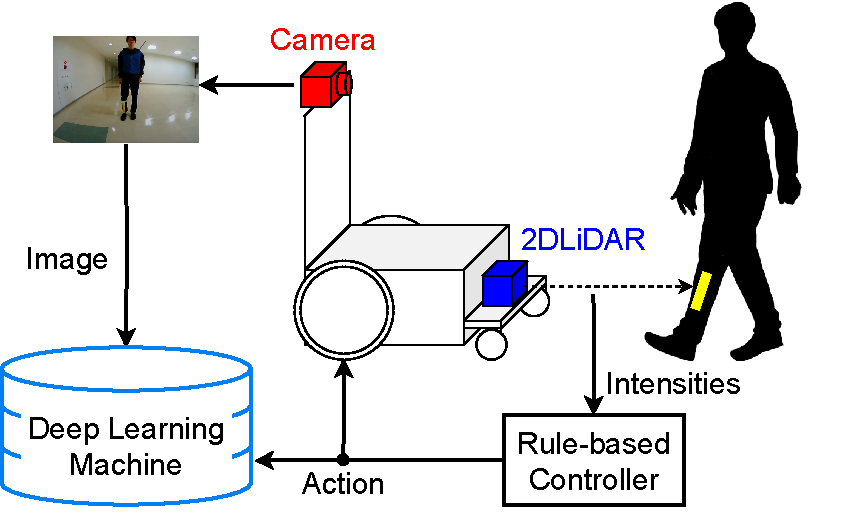
\includegraphics[keepaspectratio, scale=0.45] {images/pdf/RobotGuidance_learning_system}
    \captionsetup{justification=raggedright} % キャプションを左寄せに
    \caption{Proposed method in the learning phase}
    \label{Fig:RobotGuidance_learning_system}
  \end{figure}

  \begin{figure}[h]
    \centering
    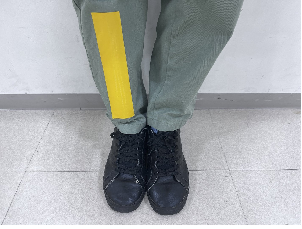
\includegraphics[keepaspectratio, scale=0.55] {images/pdf/RobotGuidance_learning_phase_leg}
    \captionsetup{justification=raggedright} % キャプションを左寄せに
    \caption{Wearing retroreflective tape}
    \label{Fig:RobotGuidance_learning_phase_leg}
  \end{figure}

\newpage

%!TEX root = ../thesis.tex

\section{追従フェーズ}

  追従フェーズの概要を\figref{Fig:RobotGuidance_following_system}に示す.追従フェーズでは,学習フェーズで獲得したモデルを用いる.ここでは,2DLiDARを使用せず,代わりに深層学習器の出力がロボットの行動に影響を与える.つまり,2DLiDARの反射強度に基づくルールベース制御器の出力ではなく,画像を入力とした深層学習器の出力がロボットの行動を決定する.

  \vspace{0.5cm}

  \begin{figure}[h]
    \centering
    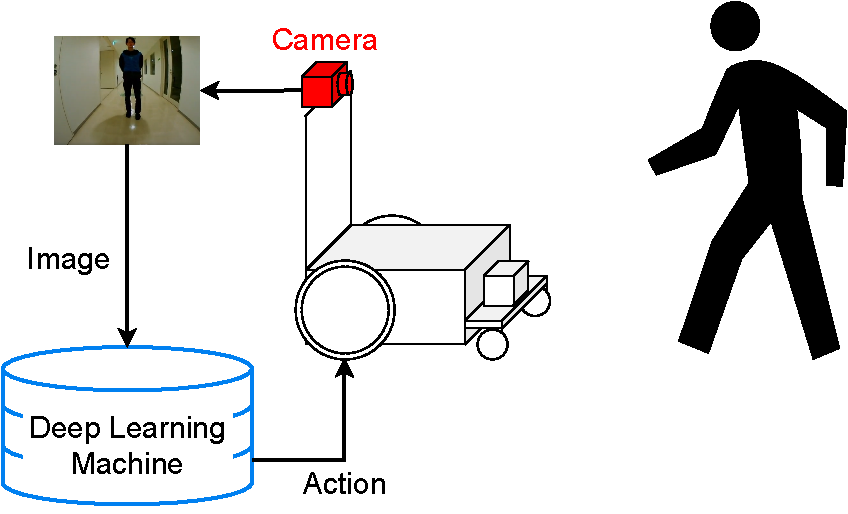
\includegraphics[keepaspectratio, scale=0.45] {images/pdf/RobotGuidance_test_system}
    \captionsetup{justification=raggedright} % キャプションを左寄せに
    \caption{Proposed method in the test phase}
    \label{Fig:RobotGuidance_following_system}
  \end{figure}

  \vspace{0.5cm}

  \begin{figure}[h]
    \centering
    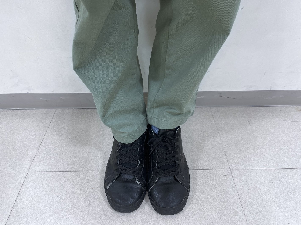
\includegraphics[keepaspectratio, scale=0.55] {images/pdf/RobotGuidance_test_phase_leg}
    \captionsetup{justification=raggedright} % キャプションを左寄せに
    \caption{Without retroreflective tape}
    \label{Fig:RobotGuidance_following_phase_leg}
  \end{figure}

\newpage

%!TEX root = ../thesis.tex

\section{反射強度を計測する装置}

  本研究で使用した2DLiDARは北陽電機社製のUTM-30LX\cite{hokuyo}である.このセンサは,ROS上で提供されている\texttt{urg\_node}\cite{urg_node}というパッケージを使用することでデータの取得ができる.この2DLiDARは,物体までの距離情報だけでなく,物体の反射強度の値も取得可能である.基本的には,\texttt{urg\_node}で提供されているデフォルトのパラメータを使用するが,\tabref{tab:parameters_of_urg_node}に示すように一部のパラメータを変更している.このセンサ自体の最大検出範囲は270 \,[deg]であるが,反射強度モードを使用する際には最大検出範囲を120 \,[deg]に制限することが推奨されている\cite{urg_node}.そのため,センサの正面を0 \,[deg]としたときに,左側に60 \,[deg](1.047 \,[rad]),右側に-60 \,[deg](-1.047 \,[rad])とした.また,1回のスキャンは25 \,[ms]時間がかかり,-60 \,[deg]から0 \,[deg]を通り60 \,[deg]に向かってレーザが回転する.この動作を\figref{Fig:Image of scan}に示す.

  \begin{table}[hbtp]
    \caption{Parameters of \texttt{urg\_node}}
    \label{tab:parameters_of_urg_node}
    \centering
    \begin{tabular}{c|cc}
    \hline
    Parameter name & Default & Experiment \\ 
    \hline
    \hline
    intensities & false   & true         \\ 
    angle\_min  & -       & -1.047       \\ 
    angle\_max  & -       & 1.047        \\ 
    \hline
    \end{tabular}
    \end{table}

    \vspace{-0.5cm}

    \begin{figure}[h]
      \centering
      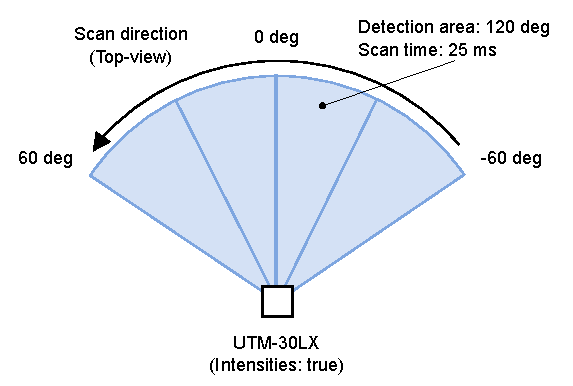
\includegraphics[height=5.5cm] {images/pdf/RobotGuidance_hokuyo_scan}
      \captionsetup{justification=raggedright} % キャプションを左寄せに
      \caption{Condition of scan}
      \label{Fig:Image of scan}
    \end{figure}

\newpage
%!TEX root = ../thesis.tex

\section{ルールベース制御器}

  学習フェーズで使用するルールベース制御器は,前節で述べた2DLiDARの反射強度を利用しており,最大反射強度の方にロボットが追従する手法となっている.この制御器の出力は,ロボットのヨ―方向の角速度$\omega$の1つであり,角速度$\omega$が0 \,[rad/s] となるようにロボットを制御する.角速度$\omega$は,以下の式\eqref{eq:angular_velocity}で表され,角度に応じた角速度$\omega$が式\eqref{eq:inequality}の範囲で出力される.

  \begin{equation}
    \omega[\text{rad/s}] = \frac{1}{\theta_{\text{max}}} \times \theta
    \label{eq:angular_velocity}
    \end{equation}

  \begin{equation}
    1 \geq \omega \geq -1
    \label{eq:inequality}
    \end{equation}

  ルールベース制御器からの出力を\tabref{tab:output_from_rule-based_controllers}に示す.ここでは,わかりやすくするために行動を左旋回,直進,右旋回の3つに分解しているが,実際に出力される行動はロボットのヨ―方向の角速度$\omega$の1つであることに注意する.

  \begin{table}[h]
    \caption{Output from rule-based controllers}
    \label{tab:output_from_rule-based_controllers}
    \begin{tabular}{|c|c|c|c|}
    \hline
    Action & Control rule {[}rad{]} & Linear velocity {[}m/s{]} & Angular velocity {[}rad/s{]} \\ 
    \hline
    Turn Left & $\text{angle\_max} \geq \theta > 0$ & 0.2 & $1 \geq \omega > 0$ \\ 
    \hline
    Forward & $0$ & 0.2 & $0$ \\ 
    \hline
    Turn Right & $0 < \theta \leq \text{angle\_min}$ & 0.2 & $0 > \omega \geq -1$ \\ 
    \hline
    \end{tabular}
    \end{table}

\newpage

  ルールベース制御器によるロボットの行動を\figref{Fig:RobotGuidance_learning_turn_left}と\figref{Fig:RobotGuidance_learning_turn_right}に示す.これは,RVizで部分的に可視化したもので,右足に装着した再帰反射テープに反応し,最大反射強度として周辺の色(黄色)とは異なる色(紫色)で表示している.
  
  \figref{Fig:RobotGuidance_learning_turn_left}の(a)は,2DLiDARの左前方にいる人(再帰反射テープ)を検出し,その角度に応じた角速度$\omega$の値が出力され,左旋回する.その結果,(b)のように角速度$\omega$はほぼ0 \,[rad/s]に近づき,直進する.

  \figref{Fig:RobotGuidance_learning_turn_right}の(a)は,2DLiDARの右前方にいる人(再帰反射テープ)を検出し,その角度に応じた角速度$\omega$の値が出力され,右旋回する.その結果,(b)のように角速度$\omega$はほぼ0 \,[rad/s]に近づき,直進する.

\begin{figure}[h]
  \centering
  \begin{minipage}[c]{65mm} 
      \centering
      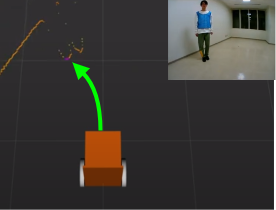
\includegraphics[height=40mm]{images/RobotGuidance_learning_turn_left_(a).png}
      \subcaption{Turn left}
  \end{minipage}
  \begin{minipage}[c]{65mm} 
      \centering
      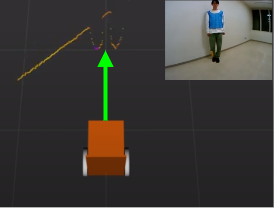
\includegraphics[height=40mm]{images/RobotGuidance_learning_turn_left_(b).png}
      \subcaption{Forward}
  \end{minipage}
  \caption{Turn left toward the retroreflective tape}
  \label{Fig:RobotGuidance_learning_turn_left}
\end{figure}

\begin{figure}[h]
  \centering
  \begin{minipage}[c]{65mm} 
      \centering
      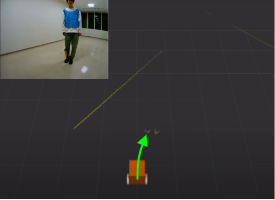
\includegraphics[height=40mm]{images/RobotGuidance_learning_turn_right_(a).png}
      \subcaption{Turn right}
  \end{minipage}
  \begin{minipage}[c]{65mm} 
      \centering
      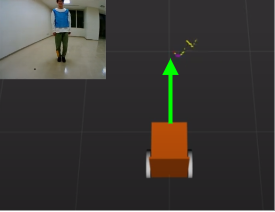
\includegraphics[height=40mm]{images/RobotGuidance_learning_turn_right_(b).png}
      \subcaption{Forward}
  \end{minipage}
  \caption{Turn right toward the retroreflective tape}
  \label{Fig:RobotGuidance_learning_turn_right}
\end{figure}

\newpage

%!TEX root = ../thesis.tex

\section{ネットワーク構造}

  ネットワークを\figref{Fig:RobotGuidance_network}に示す.これは,深層学習フレームワークであるPyTorch\cite{pytorch}を使用し,CNNをベースとしている.具体的には,入力層,畳み込み層3,全結合層2,出力層の7層で構成している.深層学習器は,縮小された画像と選択された行動を0.2秒周期で収集して学習する.これを1stepとする.使用したハイパーパラメータを\tabref{tab:Parameters of network configured with pytorch}に示す.

  \begin{figure}[h]
    \centering
    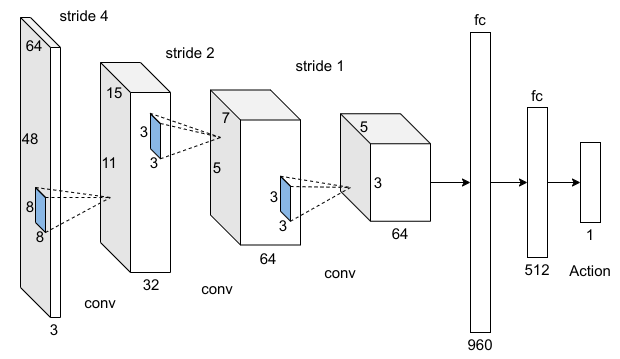
\includegraphics[keepaspectratio, scale=0.60] {images/RobotGuidance_network.png}
    \caption{Architecture of the network}
    \label{Fig:RobotGuidance_network}
  \end{figure}

  \begin{table}[hbtp]
    \caption{Parameters of network configured with PyTorch}
    \label{tab:Parameters of network configured with pytorch}
    \centering
    \begin{tabular}{cc}
      \hline
      Input data & Image(64x48 pixels, RGB channels) \\
      Optimizer & Adam($alpha = 0.001, beta1 = 0.9, beta2 =  0.999, eps = 1e^{-2}$)\\
      Loss function & Softmax-cross-entropy\\
      Output data & Angular velocity\\
      \hline
    \end{tabular}
  \end{table}

\newpage


%

\chapter{実験}
\label{chap:experiments}
%
%!TEX root = ../thesis.tex

\section{実験の手順}

\newpage

%!TEX root = ../thesis.tex

\section{実験装置}

  本研究で使用した実験装置を\figref{Fig:RobotGuidance_experiment_device}に示す.ハードウェアは,T-frogプロジェクトのi-Cart\ mini\cite{t-flog}をベースとしたロボット,ORNE-box\cite{orne-box1}\cite{orne-box2}を使用する.このロボットは,拡張性に優れており,センサの取り付け位置を自由に変えられる.よって,カメラを上部のハンドル部分に,2DLiDARを下部の足元付近に設置した.PCの仕様を\tabref{tab:Laptop specifications}に示す.また,ソフトウェアはROSを用いて構築している.深層学習のフレームワークには,PyTorchを用いている.

  \begin{figure}[h]
    \centering
    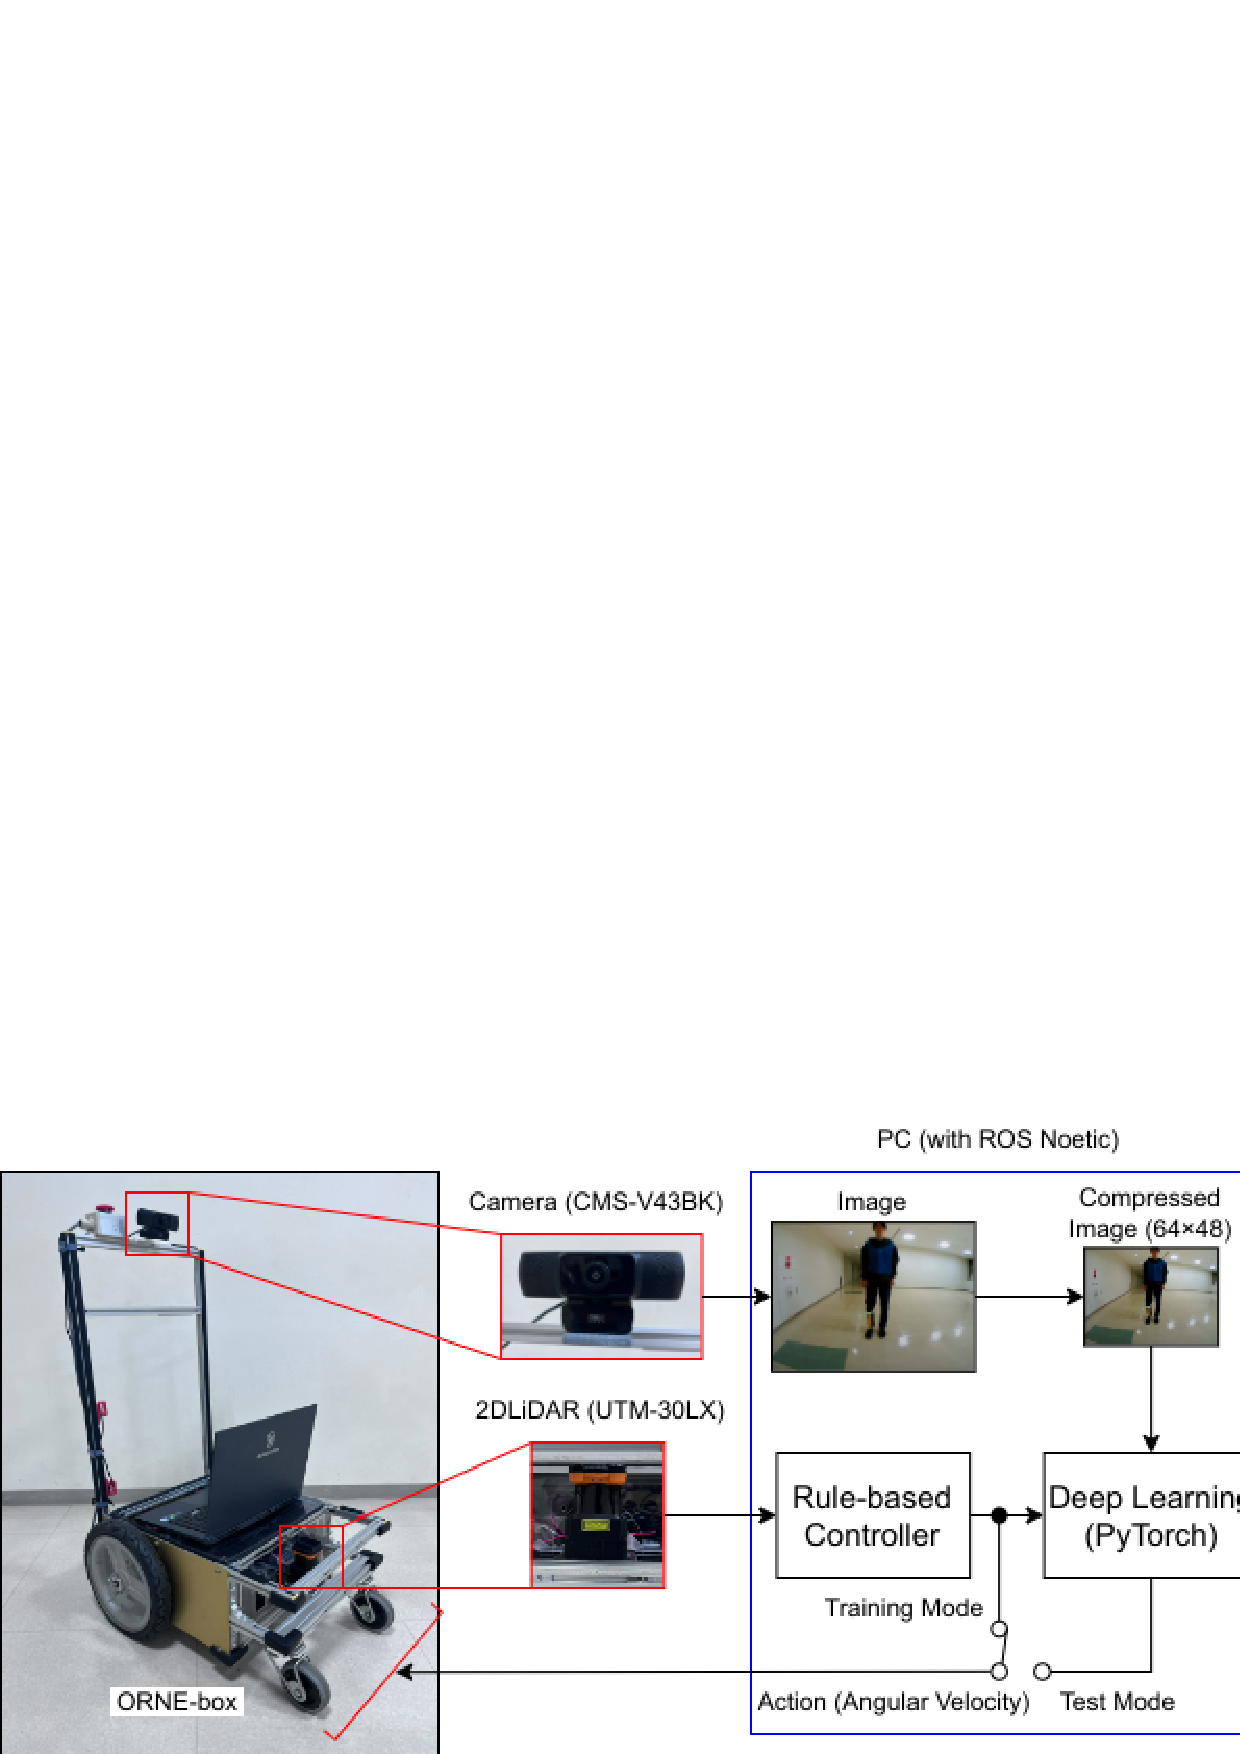
\includegraphics[keepaspectratio, scale=0.60] {images/RobotGuidance_experiment_device.png}
    \captionsetup{justification=raggedright} % キャプションを左寄せに
    \caption{The developed system}
    \label{Fig:RobotGuidance_experiment_device}
  \end{figure}

  \begin{table}[h]
    \caption{Laptop specifications}
    \label{tab:Laptop specifications}
    \centering
    \begin{tabular}{|c|c|}
    \hline
    Processor & Spec                               \\ \hline
    OS   & Ubuntu 20.04 LTS                        \\ \hline
    ROS  & Noetic                                  \\ \hline
    CPU  & intel Core i7-10700F(4.8GHz/8コア/16スレッド) \\ \hline
    GPU  & RTX 2070 Max-Q                          \\ \hline
    DRAM & 32GB DDR4(3200/8GB × 4)                 \\ \hline
    \end{tabular}
    \end{table}

\newpage

%!TEX root = ../thesis.tex

\section{実験1:2DLiDARの反射強度の実験}

  実験1では,2DLiDARの反射強度を利用した実験を行う.ここでは,以下に示す3つの事項に関して調査する.なお,以下の実験では,2DLiDARの検出範囲を0 \,[rad]で更に制限している.
  % 4の実験では,提案手法通り最大2.094 \,[rad](120 \,[deg])の範囲で検出する.

  \begin{enumerate}
    \item 壁の反射強度を計測する実験
    \item 再帰反射テープの反射強度を計測する実験
    \item 学習フェーズで使用する周辺環境の反射強度を計測する実験
    % \item ルールベース制御器を用いた人追従の実験
  \end{enumerate}

\subsection{実験目的}

本研究では,2DLiDARの反射強度を利用したルールベース制御器を用いた人追従行動を,カメラ画像で模倣学習することを課題としている.ルールベース制御器は,最大反射強度の方にロボットが追従する手法となっているため,実験で使用する再帰反射テープよりも高い反射強度を取得してしまうと人追従行動を継続できない恐れがある.そのため,実験場所として指定した,千葉工業大学津田沼キャンパス2号館3階の廊下において,再帰反射テープよりも反射強度の高いものが存在しないかを,実験により調査する.

\newpage

\subsection{壁の反射強度}

  実験場所である,千葉工業大学津田沼キャンパス2号館3階の廊下の壁の反射強度を計測した.実験の様子を\figref{Fig:RobotGuidance_exp1_wall}に示す.2DLiDARを壁に向けて正面に配置し,距離によって反射強度の値が変化するのを防ぐため,壁から約500 \,[mm]離れたところに固定した.
  
  計測した結果を\figref{Fig:Normal distribution of reflection intensity of wall}に示す.収集したデータは1万個で,平均値は約3600であり,平均値付近にデータが集中していることがわかった.

  \begin{figure}[h]
    \centering
    \begin{minipage}[c]{65mm} 
        \centering
        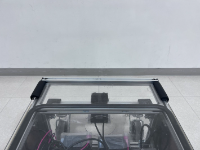
\includegraphics[height=40mm]{images/RobotGuidance_exp1_wall_from_back.png}
        \subcaption{View from behind}
    \end{minipage}
    \begin{minipage}[c]{65mm} 
        \centering
        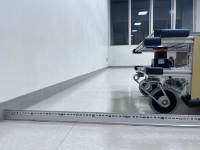
\includegraphics[height=40mm]{images/RobotGuidance_exp1_wall_from_side.png}
        \subcaption{View from the side}
    \end{minipage}
    \caption{Measure the reflection intensity of the wall}
    \label{Fig:RobotGuidance_exp1_wall}
  \end{figure}

  \begin{figure}[h]
    \centering
    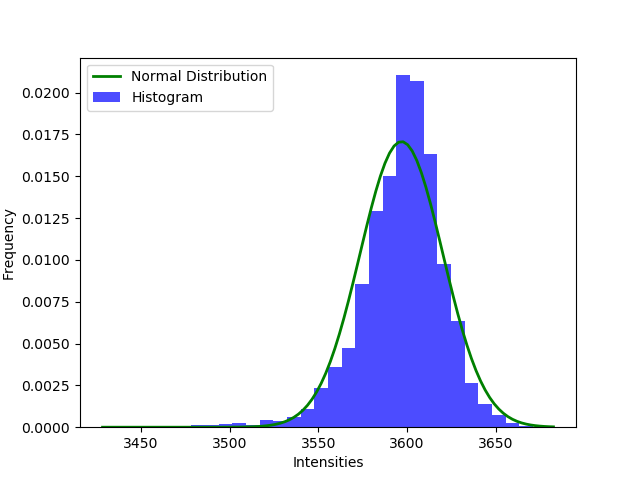
\includegraphics[keepaspectratio, scale=0.50] {images/RobotGuidance_plot_reflection_intensities_of_wall.png}
    \captionsetup{justification=raggedright} % キャプションを左寄せに
    \caption{Normal distribution of reflection intensity of wall}
    \label{Fig:Normal distribution of reflection intensity of wall}
  \end{figure}

\newpage

\subsection{再帰反射テープの反射強度}

  再帰反射テープの反射強度を計測した.実験の様子を\figref{Fig:RobotGuidance_exp2_tape}に示す.2DLiDARを再帰反射テープに向けて正面に配置し,距離によって反射強度の値が変化するのを防ぐため,再帰反射テープから約500 \,[mm]離れたところに固定した.
    
  計測した結果を\figref{Fig:Normal distribution of reflection intensity of retroreflective tape}に示す.収集したデータは1万個で,平均値は約15300であり,平均値付近にデータが集中していることがわかった.

  \begin{figure}[h]
    \centering
    \begin{minipage}[c]{65mm} 
        \centering
        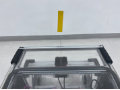
\includegraphics[height=40mm]{images/RobotGuidance_exp2_tape_from_back.png}
        \subcaption{View from behind}
    \end{minipage}
    \begin{minipage}[c]{65mm} 
        \centering
        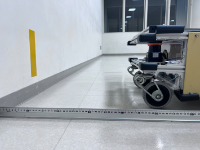
\includegraphics[height=40mm]{images/RobotGuidance_exp2_tape_from_side.png}
        \subcaption{View from the side}
    \end{minipage}
    \caption{Measure the reflection intensity of retroreflective tape}
    \label{Fig:RobotGuidance_exp2_tape}
  \end{figure}

  \begin{figure}[h]
    \centering
    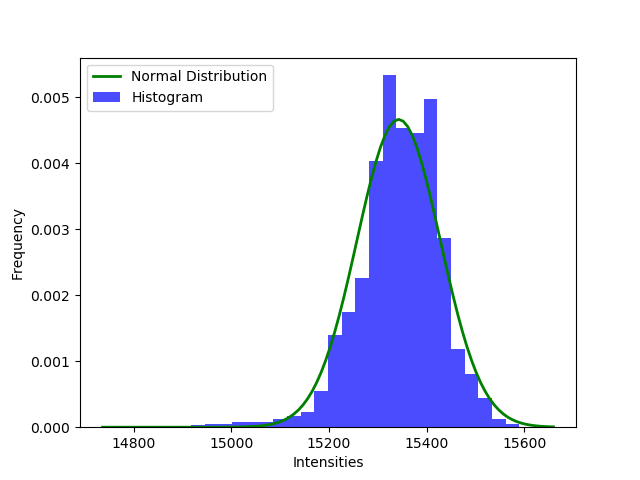
\includegraphics[keepaspectratio, scale=0.50] {images/RobotGuidance_plot_reflection_intensities_of_tape.png}
    \captionsetup{justification=raggedright} % キャプションを左寄せに
    \caption{Normal distribution of reflection intensity of retroreflective tape}
    \label{Fig:Normal distribution of reflection intensity of retroreflective tape}
  \end{figure}

\newpage

\subsection{学習する場所付近の反射強度}

  学習フェーズで使用する場所を\figref{Fig:RobotGuidance_exp3_foyer}に示す.ここは,千葉工業大学津田沼キャンパス2号館3階のホワイエと呼ばれるスペースであり,中にはガラスや自動販売機が存在する.それぞれに対して反射強度を計測するのは大変なので,ホワイエをランダムに歩き回ることでデータを収集する.

  計測した結果を\figref{Fig:Histogram of reflection intensity of foyer}に示す.収集したデータは1万個で,ホワイエには5000を超える反射強度の値は存在しないことがわかった.つまり,再帰反射テープが最大反射強度であり,ルールベース制御器が正常に機能すると,人追従行動生成が可能であることを確認した.

  \begin{figure}[h]
    \centering
    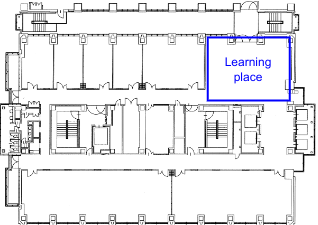
\includegraphics[keepaspectratio, scale=0.50] {images/RobotGuidance_exp3_foyer.png}
    \captionsetup{justification=raggedright} % キャプションを左寄せに
    \caption{Measure the reflection intensity of foyer}
    \label{Fig:RobotGuidance_exp3_foyer}
  \end{figure}

  \begin{figure}[h]
    \centering
    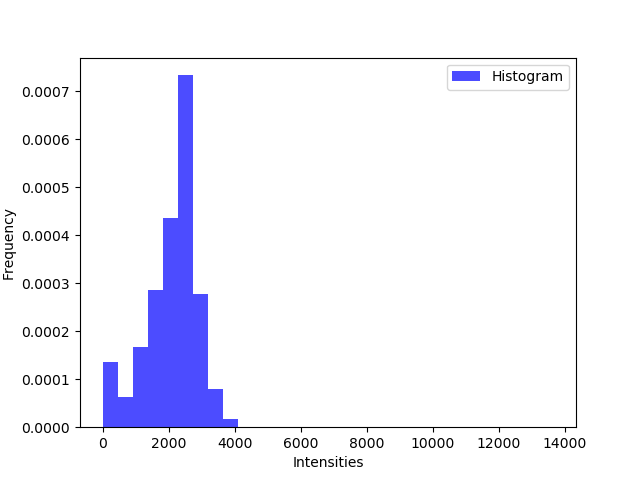
\includegraphics[keepaspectratio, scale=0.50] {images/RobotGuidance_plot_reflection_intensities_of_foyer.png}
    \captionsetup{justification=raggedright} % キャプションを左寄せに
    \caption{Histogram of reflection intensity of foyer}
    \label{Fig:Histogram of reflection intensity of foyer}
  \end{figure}

\newpage

% \subsection{反射強度を利用した人追従の実験}

%   2DLiDARの反射強度を利用した人追従の実験を行う.この実験により,ルールベース制御器がホワイエにて有効であるか明らかにする.実験の様子を\figref{Fig:Parson following behavior using rule-based controller}に示す.10分間,ホワイエをランダムに歩き回り,その間のルールベース制御器によるロボットの挙動を観察した.その結果,ロボットはルールベース制御器に従い,10分間にわたり人を追従し続け,その有効性を確認した.

%   \begin{figure}[h]
%     \centering
%     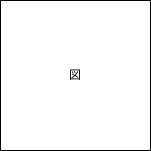
\includegraphics[keepaspectratio, scale=0.80] {images/figure.png}
%     \captionsetup{justification=raggedright} % キャプションを左寄せに
%     \caption{Parson following behavior using rule-based controller}
%     \label{Fig:Parson following behavior using rule-based controller}
%   \end{figure}

% \newpage

%!TEX root = ../thesis.tex
\section{実験2:提案手法による人追従の実験}

  実験2では,提案手法による人追従の実験を行う.

\subsection{実験目的}

  提案手法により画像に基づいて人を追従する行動が生成されるかを,10回の実験により有効性を検証する.

\subsection{実験方法}

  実験では,学習フェーズの後に追従フェーズに移行する.以下にそれぞれの役割を示す.

  \subsubsection*{<学習フェーズ>}
  学習フェーズでは,追従対象者が再帰反射テープを装着し,\figref{Fig:RobotGuidance_course}における青色で示された場所(ホワイエ)を2DLiDARの最大検出範囲(120\, [deg])に注意しながら,10分間ランダムに歩き回る.

  \subsubsection*{<追従フェーズ>}
  追従フェーズでは,反射強度を利用していないことをわかりやすくするため,追従対象者は再帰反射テープを取り外す.また,学習フェーズとは異なり,\figref{Fig:RobotGuidance_course}における赤色で示されたコースを1周する.このコースは1周約90mであり,学習フェーズで学習したモデルを用いて,2DLiDARは使用せずに画像のみで人追従を行う.その時のロボットの挙動を確認する.

  \vspace{1cm}

  学習フェーズでの10分間の学習と追従フェーズでのテストコースを1周することを1セットとし,10セット実験を行った.

\newpage

  \begin{figure}[h]
    \centering
    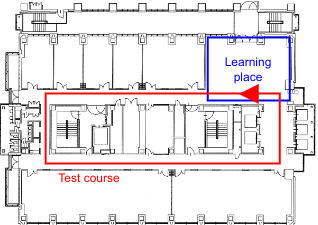
\includegraphics[keepaspectratio, scale=0.70] {images/RobotGuidance_course.png}
    \captionsetup{justification=raggedright} % キャプションを左寄せに
    \caption{Learning and following phase courses}
    \label{Fig:RobotGuidance_course}
  \end{figure}

\newpage

\subsection{結果と考察}

  すべての実験でロボットが人を追従する様子が確認できた.以下にそれぞれのフェーズの様子を記述する.

  \subsubsection*{<学習フェーズ>}
  
  学習フェーズにおける実験の様子を\figref{Fig:Learning phase in experiment}に示す.2DLiDARの反射強度を利用したルールベース制御器を使用することで学習フェーズにおいてロボットが人を追従する様子が確認できた.10セットの学習を行ったが,全てのセットにおいて人追従が途切れることはなかった.つまり,ルールベース制御器の有効性が確認できた.

  \begin{figure}[h]
    \centering
    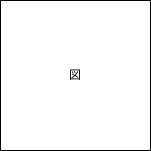
\includegraphics[keepaspectratio, scale=0.80] {images/figure.png}
    \captionsetup{justification=raggedright} % キャプションを左寄せに
    \caption{Learning phase in experiment}
    \label{Fig:Learning phase in experiment}
  \end{figure}

\newpage

  \subsubsection*{<追従フェーズ>}
  
  追従フェーズにおける実験の様子を\figref{Fig:Following phase in experiment}に示す.テストコースの道中で,追従対象者のビブスと同じ青色の壁紙が貼られていたが,そちらに釣られることなく人追従行動を継続する様子が確認できた.

  \begin{figure}[h]
    \centering
    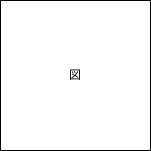
\includegraphics[keepaspectratio, scale=0.80] {images/figure.png}
    \captionsetup{justification=raggedright} % キャプションを左寄せに
    \caption{Following phase in experiment}
    \label{Fig:Following phase in experiment}
  \end{figure}

  実験結果を\figref{tab:Experiment result}に示す.10回の試行中,9回は壁に衝突することなくコースを1周することができた.学習ステップ数は,0.2秒周期で学習して1stepとしているので,10分の学習で3000stepとなった.つまり,各学習モデルには3000個のデータが含まれ,人追従行動を明示的に学習せずに自動的に獲得している.一方で,10回の試行中,1回は\figref{Fig:RobotGuidance_failed_place}に示すように,テストコースの最初の曲がり角で壁に衝突した.失敗した場合の学習フェーズでの角速度のヒストグラムを\figref{Fig:Histogram of angular velocity}の(b)に示す.成功時の角速度のヒストグラムは(a)で,両者を比較すると,失敗時の左旋回の最大角速度が0.1\, [rad/s]小さいことがわかる.このことから,学習フェーズで0.3\, [rad/s]以上の角速度で左旋回する行動を学習していないのにもかかわらず,追従フェーズで0.3\, [rad/s]以上の角速度で左旋回しなければならない位置に追従対象者が立っていたことが原因で,曲がりきれずに壁に衝突してしまったと考えられる.ただし,これについてはさらなる調査が必要である.

  \begin{table}[h]
    \caption{Experiment result}
    \label{tab:Experiment result}
    \centering
    \begin{tabular}{|c|c|}
    \hline
    Step & Result      \\ \hline
    3000 & 9/10 (90\%) \\ \hline
    \end{tabular}
    \end{table}

\newpage

  \begin{figure}[h]
    \centering
    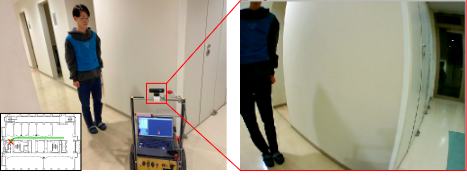
\includegraphics[keepaspectratio, scale=0.80] {images/RobotGuidance_failed_place.png}
    \captionsetup{justification=raggedright} % キャプションを左寄せに
    \caption{Failed at the first corner}
    \label{Fig:RobotGuidance_failed_place}
  \end{figure}

  \begin{figure}[h]
    \centering
    \begin{minipage}[c]{65mm} 
        \centering
        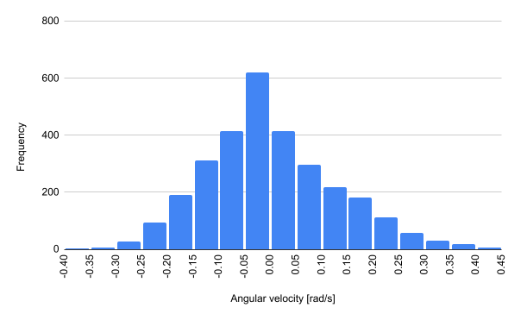
\includegraphics[height=45mm]{images/RobotGuidance_success_histogram.png}
        \subcaption{Success}
    \end{minipage}
    \begin{minipage}[c]{65mm} 
        \centering
        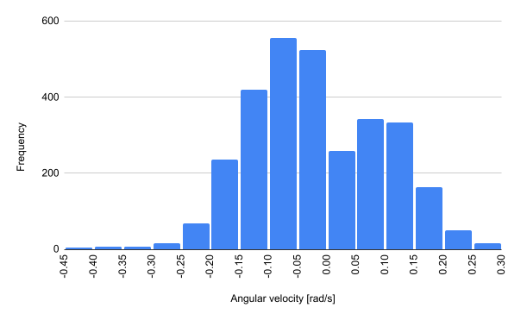
\includegraphics[height=45mm]{images/RobotGuidance_failed_histogram.png}
        \subcaption{Failure}
    \end{minipage}
    \caption{Histogram of angular velocity}
    \label{Fig:Histogram of angular velocity}
  \end{figure}

\newpage


%

\chapter{結論}
\label{end}
%
%!TEX root = ../thesis.tex

\section{Deep Learning}

\newpage

%

%
%% Back Matter
\backmatter{}
%
\chapter{提案手法}

  本章では,従来手法をベースとする提案手法の概要,提案手法における学習フェーズ,追従フェーズ,ルールベース制御器,ネットワーク構造についての5節に分けて述べる.

\label{chap:suggest}
%
%!TEX root = ../thesis.tex

\section{提案手法の概要}

  本研究は,ルールベース制御器の入力に引き紐ではなく,2DLiDARの反射強度を利用する.このときのロボットの行動を\figref{Fig:RobotGuidance_velocity}に示す.並進速度は,学習時と学習後で共に0.2 \,[m/s]で一定であり,ロボットのヨ―方向の角速度$\omega$のみが変化する.ルールベース制御器は,反射強度の高い方向にロボットを追従させる制御で,追従対象者に再帰反射テープを装着し,2DLiDARでそれを検出することで,人に追従する手法である.

  \begin{figure}[h]
    \centering
    \begin{minipage}[c]{65mm} 
        \centering
        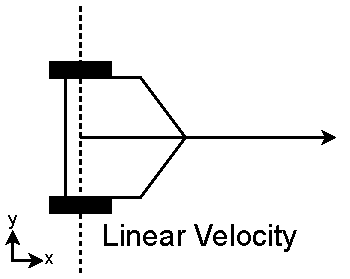
\includegraphics[height=40mm]{images/pdf/RobotGuidance_linear_velocity}
        \subcaption{Forward is fixed}
    \end{minipage}
    \begin{minipage}[c]{65mm} 
        \centering
        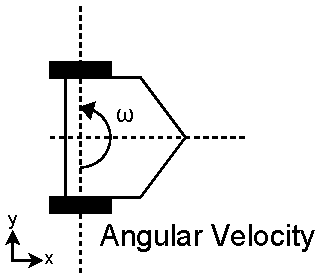
\includegraphics[height=40mm]{images/pdf/RobotGuidance_angular_velocity}
        \subcaption{Angular velocity changes depending on input}
    \end{minipage}
    \caption{Output robot actions}
    \label{Fig:RobotGuidance_velocity}
  \end{figure}

\newpage

  深層学習器は,ルールベース制御器の出力(ロボットのヨ―方向の角速度$\omega$)とRGB画像をend-to-end学習することで,\figref{Fig:RobotGuidance_simple_system}に示すように,入力をRGB画像,出力をロボットのヨ―方向の角速度$\omega$として人を追従する.

  \begin{figure}[h]
    \centering
    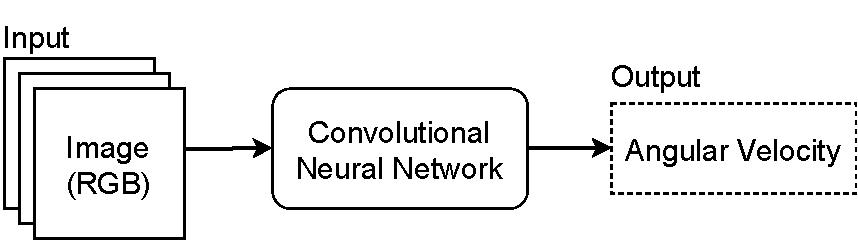
\includegraphics[height=3cm] {images/pdf/RobotGuidance_simple_system}
    \captionsetup{justification=raggedright} % キャプションを左寄せに
    \caption{The trained network is used to generate the robot's yaw angular velocity from the RGB images}
    \label{Fig:RobotGuidance_simple_system}
  \end{figure}

  \figref{Fig:RobotGuidance_all_system}に示すように,ルールベース制御器を用いてロボットを制御するフェーズを学習フェーズ,深層学習器の出力をロボットの行動にするフェーズをテストフェーズと呼ぶこととする.以下に,学習フェーズとテストフェーズの主な役割を示す.

  \subsubsection*{<学習フェーズ>}
  2DLiDARの反射強度を利用したルールベース制御器に従い,ロボットを制御する.制御器の出力と画像を教師信号として深層学習器に与え,オンラインでend-to-end学習する.
  
  \subsubsection*{<テストフェーズ>}
  2DLiDARは使用せず,画像を入力とした深層学習器の出力をロボットの行動にする.画像に基づいた人追従ができるかを実験により確認する.

  \begin{figure}[h]
    \centering
    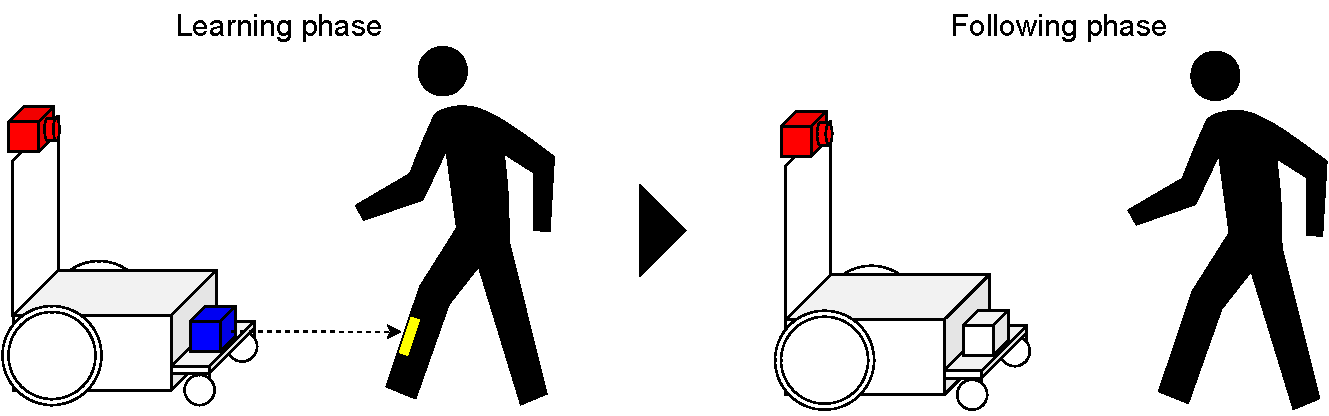
\includegraphics[height=3.5cm] {images/pdf/RobotGuidance_all_system}
    \captionsetup{justification=raggedright} % キャプションを左寄せに
    \caption{Sequence of proposed method}
    \label{Fig:RobotGuidance_all_system}
  \end{figure}

\newpage

%!TEX root = ../thesis.tex

\section{学習フェーズ}

  学習フェーズの概要を\figref{Fig:RobotGuidance_learning_system}に示す.学習フェーズでは,2DLiDARの反射強度を利用したルールベース制御器を用いて,\figref{Fig:RobotGuidance_learning_phase_leg}に示す追従対象者の足に装着した再帰反射テープに向かって,ロボットを制御する.ルールベース制御器の出力は,ロボットのヨ―方向の角速度$\omega$の1つとし,角速度$\omega$が0 \,[rad/s]となるようにロボットを制御することで人追従することが可能と考えられる.並行して,この行動とカメラの画像データを深層学習器に入力して,オンラインで学習させる.なお,並進速度は0.2 \,[m/s]で一定にしているため,深層学習器に入力しない.

  \begin{figure}[h]
    \centering
    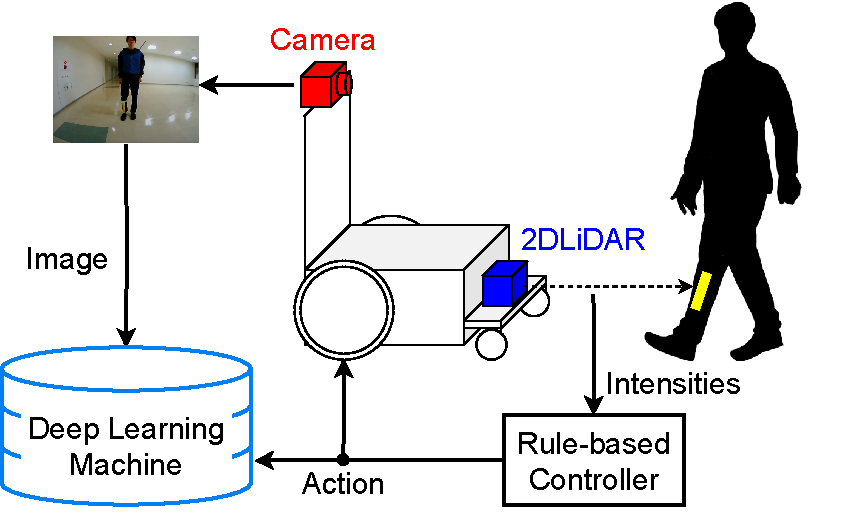
\includegraphics[keepaspectratio, scale=0.45] {images/pdf/RobotGuidance_learning_system}
    \captionsetup{justification=raggedright} % キャプションを左寄せに
    \caption{Proposed method in the learning phase}
    \label{Fig:RobotGuidance_learning_system}
  \end{figure}

  \begin{figure}[h]
    \centering
    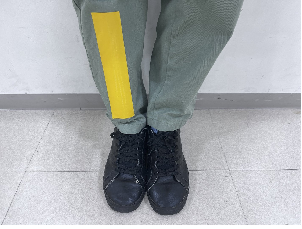
\includegraphics[keepaspectratio, scale=0.55] {images/pdf/RobotGuidance_learning_phase_leg}
    \captionsetup{justification=raggedright} % キャプションを左寄せに
    \caption{Wearing retroreflective tape}
    \label{Fig:RobotGuidance_learning_phase_leg}
  \end{figure}

\newpage

%!TEX root = ../thesis.tex

\section{追従フェーズ}

  追従フェーズの概要を\figref{Fig:RobotGuidance_following_system}に示す.追従フェーズでは,学習フェーズで獲得したモデルを用いる.ここでは,2DLiDARを使用せず,代わりに深層学習器の出力がロボットの行動に影響を与える.つまり,2DLiDARの反射強度に基づくルールベース制御器の出力ではなく,画像を入力とした深層学習器の出力がロボットの行動を決定する.

  \vspace{0.5cm}

  \begin{figure}[h]
    \centering
    \includegraphics[keepaspectratio, scale=0.45] {images/pdf/RobotGuidance_test_system}
    \captionsetup{justification=raggedright} % キャプションを左寄せに
    \caption{Proposed method in the test phase}
    \label{Fig:RobotGuidance_following_system}
  \end{figure}

  \vspace{0.5cm}

  \begin{figure}[h]
    \centering
    \includegraphics[keepaspectratio, scale=0.55] {images/pdf/RobotGuidance_test_phase_leg}
    \captionsetup{justification=raggedright} % キャプションを左寄せに
    \caption{Without retroreflective tape}
    \label{Fig:RobotGuidance_following_phase_leg}
  \end{figure}

\newpage

%!TEX root = ../thesis.tex

\section{反射強度を計測する装置}

  本研究で使用した2DLiDARは北陽電機社製のUTM-30LX\cite{hokuyo}である.このセンサは,ROS上で提供されている\texttt{urg\_node}\cite{urg_node}というパッケージを使用することでデータの取得ができる.この2DLiDARは,物体までの距離情報だけでなく,物体の反射強度の値も取得可能である.基本的には,\texttt{urg\_node}で提供されているデフォルトのパラメータを使用するが,\tabref{tab:parameters_of_urg_node}に示すように一部のパラメータを変更している.このセンサ自体の最大検出範囲は270 \,[deg]であるが,反射強度モードを使用する際には最大検出範囲を120 \,[deg]に制限することが推奨されている\cite{urg_node}.そのため,センサの正面を0 \,[deg]としたときに,左側に60 \,[deg](1.047 \,[rad]),右側に-60 \,[deg](-1.047 \,[rad])とした.また,1回のスキャンは25 \,[ms]時間がかかり,-60 \,[deg]から0 \,[deg]を通り60 \,[deg]に向かってレーザが回転する.この動作を\figref{Fig:Image of scan}に示す.

  \begin{table}[hbtp]
    \caption{Parameters of \texttt{urg\_node}}
    \label{tab:parameters_of_urg_node}
    \centering
    \begin{tabular}{c|cc}
    \hline
    Parameter name & Default & Experiment \\ 
    \hline
    \hline
    intensities & false   & true         \\ 
    angle\_min  & -       & -1.047       \\ 
    angle\_max  & -       & 1.047        \\ 
    \hline
    \end{tabular}
    \end{table}

    \vspace{-0.5cm}

    \begin{figure}[h]
      \centering
      \includegraphics[height=5.5cm] {images/pdf/RobotGuidance_hokuyo_scan}
      \captionsetup{justification=raggedright} % キャプションを左寄せに
      \caption{Condition of scan}
      \label{Fig:Image of scan}
    \end{figure}

\newpage
%!TEX root = ../thesis.tex

\section{ルールベース制御器}

  学習フェーズで使用するルールベース制御器は,前節で述べた2DLiDARの反射強度を利用しており,最大反射強度の方にロボットが追従する手法となっている.この制御器の出力は,ロボットのヨ―方向の角速度$\omega$の1つであり,角速度$\omega$が0 \,[rad/s] となるようにロボットを制御する.角速度$\omega$は,以下の式\eqref{eq:angular_velocity}で表され,角度に応じた角速度$\omega$が式\eqref{eq:inequality}の範囲で出力される.

  \begin{equation}
    \omega[\text{rad/s}] = \frac{1}{\theta_{\text{max}}} \times \theta
    \label{eq:angular_velocity}
    \end{equation}

  \begin{equation}
    1 \geq \omega \geq -1
    \label{eq:inequality}
    \end{equation}

  ルールベース制御器からの出力を\tabref{tab:output_from_rule-based_controllers}に示す.ここでは,わかりやすくするために行動を左旋回,直進,右旋回の3つに分解しているが,実際に出力される行動はロボットのヨ―方向の角速度$\omega$の1つであることに注意する.

  \begin{table}[h]
    \caption{Output from rule-based controllers}
    \label{tab:output_from_rule-based_controllers}
    \begin{tabular}{|c|c|c|c|}
    \hline
    Action & Control rule {[}rad{]} & Linear velocity {[}m/s{]} & Angular velocity {[}rad/s{]} \\ 
    \hline
    Turn Left & $\text{angle\_max} \geq \theta > 0$ & 0.2 & $1 \geq \omega > 0$ \\ 
    \hline
    Forward & $0$ & 0.2 & $0$ \\ 
    \hline
    Turn Right & $0 < \theta \leq \text{angle\_min}$ & 0.2 & $0 > \omega \geq -1$ \\ 
    \hline
    \end{tabular}
    \end{table}

\newpage

  ルールベース制御器によるロボットの行動を\figref{Fig:RobotGuidance_learning_turn_left}と\figref{Fig:RobotGuidance_learning_turn_right}に示す.これは,RVizで部分的に可視化したもので,右足に装着した再帰反射テープに反応し,最大反射強度として周辺の色(黄色)とは異なる色(紫色)で表示している.
  
  \figref{Fig:RobotGuidance_learning_turn_left}の(a)は,2DLiDARの左前方にいる人(再帰反射テープ)を検出し,その角度に応じた角速度$\omega$の値が出力され,左旋回する.その結果,(b)のように角速度$\omega$はほぼ0 \,[rad/s]に近づき,直進する.

  \figref{Fig:RobotGuidance_learning_turn_right}の(a)は,2DLiDARの右前方にいる人(再帰反射テープ)を検出し,その角度に応じた角速度$\omega$の値が出力され,右旋回する.その結果,(b)のように角速度$\omega$はほぼ0 \,[rad/s]に近づき,直進する.

\begin{figure}[h]
  \centering
  \begin{minipage}[c]{65mm} 
      \centering
      \includegraphics[height=40mm]{images/RobotGuidance_learning_turn_left_(a).png}
      \subcaption{Turn left}
  \end{minipage}
  \begin{minipage}[c]{65mm} 
      \centering
      \includegraphics[height=40mm]{images/RobotGuidance_learning_turn_left_(b).png}
      \subcaption{Forward}
  \end{minipage}
  \caption{Turn left toward the retroreflective tape}
  \label{Fig:RobotGuidance_learning_turn_left}
\end{figure}

\begin{figure}[h]
  \centering
  \begin{minipage}[c]{65mm} 
      \centering
      \includegraphics[height=40mm]{images/RobotGuidance_learning_turn_right_(a).png}
      \subcaption{Turn right}
  \end{minipage}
  \begin{minipage}[c]{65mm} 
      \centering
      \includegraphics[height=40mm]{images/RobotGuidance_learning_turn_right_(b).png}
      \subcaption{Forward}
  \end{minipage}
  \caption{Turn right toward the retroreflective tape}
  \label{Fig:RobotGuidance_learning_turn_right}
\end{figure}

\newpage

%!TEX root = ../thesis.tex

\section{ネットワーク構造}

  ネットワークを\figref{Fig:RobotGuidance_network}に示す.これは,深層学習フレームワークであるPyTorch\cite{pytorch}を使用し,CNNをベースとしている.具体的には,入力層,畳み込み層3,全結合層2,出力層の7層で構成している.深層学習器は,縮小された画像と選択された行動を0.2秒周期で収集して学習する.これを1stepとする.使用したハイパーパラメータを\tabref{tab:Parameters of network configured with pytorch}に示す.

  \begin{figure}[h]
    \centering
    \includegraphics[keepaspectratio, scale=0.60] {images/RobotGuidance_network.png}
    \caption{Architecture of the network}
    \label{Fig:RobotGuidance_network}
  \end{figure}

  \begin{table}[hbtp]
    \caption{Parameters of network configured with PyTorch}
    \label{tab:Parameters of network configured with pytorch}
    \centering
    \begin{tabular}{cc}
      \hline
      Input data & Image(64x48 pixels, RGB channels) \\
      Optimizer & Adam($alpha = 0.001, beta1 = 0.9, beta2 =  0.999, eps = 1e^{-2}$)\\
      Loss function & Softmax-cross-entropy\\
      Output data & Angular velocity\\
      \hline
    \end{tabular}
  \end{table}

\newpage


%

%

\end{document}
